    \documentclass[12pt,openright]{report}
    \usepackage{estilo}
    \makenomenclature

    \begin{document}
    \tolerance=5000

    %====================================================================
    %Capa
    %====================================================================
    \capa
    {ANÁLISE DE DESEMPENHO DE CORREDORES UTILIZANDO DADOS DO STRAVA: UMA ABORDAGEM DE REGRESSÃO LINEAR.}
    {João Marcos de Souza Matos}
    {2025}
    {Pedro Franklin Cardoso Silva}
    %{Nome completo do segundo membro da banca de defesa}
    %{Nome completo do terceiro membro da banca de defesa}

    %====================================================================
    % INÍCIO DOS ELEMENTOS PRÉ-TEXTUAIS
    %====================================================================
    \setcounter{page}{1} % Define manualmente o contador da página para 1

    %====================================================================
    % Agradecimentos: Os agradecimentos deverão ser escritos dentro do 
    % arquivo agradecimentos.tex. 
    %====================================================================     
    
\chapter*{Agradecimentos}
\thispagestyle{empty}


Nesta seção, desejo expressar minha profunda gratidão a todos que, de formas distintas, contribuíram para a realização deste trabalho e para minha formação acadêmica e pessoal.

Primeiramente, agradeço a Deus por me dar forças para continuar e não desistir diante das dificuldades, me proporcionando sabedoria e paciência em momentos desafiadores.

Ao meu orientador, Prof. Pedro Franklin Cardoso Silva, agradeço pela orientação, paciência e pela sua constante prontidão em me ajudar. Sua dedicação e conhecimento são inspiração para mim.

À Universidade Federal de Uberlândia e ao Instituto de Matemática e Estatística, por oferecerem um ambiente acadêmico rico e estimulante, que foi fundamental para meu crescimento intelectual.

Aos membros da banca examinadora, por aceitarem o convite de avaliar este trabalho. O tempo e conhecimento de vocês serão de grande valia para o aprimoramento deste estudo.

À Bianca Souza, que sempre esteve ao meu lado para me incentivar nos momentos de dúvida, para me erguer nas quedas e para celebrar cada conquista comigo. Você é um dos pilares mais importantes da minha vida.

Aos meus pais, Fernanda de Souza e Marco Matos, por todo amor, colo, amparo e apoio incondicional. Vocês são minha base e meu exemplo de vida.

Aos meus irmãos, Vitória, José e Antônio, por serem minha fonte de alegria.

Aos meus amigos e colegas de curso, por compartilharem essa jornada comigo, tornando-a mais leve e divertida. Alguns de vocês se tornaram verdadeiros irmãos para mim.
    \cleardoublepage

    % --- Epígrafe (Opcional) ---
    % Garante que esta página não terá cabeçalho, rodapé ou número.
\thispagestyle{empty}

% Adiciona um espaço vertical flexível que empurra todo o conteúdo
% para a parte de baixo da página.
\vspace*{\fill}

% Este ambiente alinha o bloco da epígrafe à margem DIREITA da página.
\begin{flushright}
    % Criamos uma "caixa" (minipage) com uma largura fixa.
    % Você pode ajustar o valor de 7cm para deixar a citação
    % mais larga ou mais estreita. Tente 6cm ou 8cm se desejar.
    \begin{minipage}{7cm}
        % Este comando força TODO o texto dentro da caixa
        % a ser alinhado à direita. É o segredo para juntar
        % o autor e a citação.
        \raggedleft
        
        % O texto da citação, em itálico. A dupla barra \\ cria uma nova linha.
        \textit{"Não é só correr."} \\
        
        % Adiciona um pequeno espaço vertical entre a citação e o autor.
        \vspace{0.5\baselineskip}
        
        % O nome do autor.
        --- P. Lamin
        
    \end{minipage}
\end{flushright}
\vspace*{5cm}
    \cleardoublepage
    %====================================================================
    % Resumo em português: O resumo em português
    %====================================================================
    \chapter*{Resumo}
\thispagestyle{empty}
\label{chap:resumo}

\textbf{Introdução:} A corrida de montanha tem ganhado destaque entre modalidades esportivas ao ar livre, sendo influenciada por fatores como: ritmo, desnível e inclinação. Dados de plataformas de rastreamento de atividades permitem analisar variáveis de desempenho, oferecendo uma base para compreender melhor como esses elementos impactam os resultados dos corredores.
\textbf{Objetivo:} Aplicar modelos de regressão linear múltipla para analisar o desempenho de corredores de montanha, utilizando dados coletados da plataforma Strava.
\textbf{Metodologia:} Caracteriza-se como um estudo quantitativo, de caráter descritivo e explicativo. Foi realizado um processo de engenharia de variáveis para a criação de métricas de ritmo, estratégia e performance. Subsequentemente, foi aplicada a análise de agrupamento K-Means para a identificação de perfis de corredores e ajustado um modelo de regressão linear múltipla para analisar a relação entre o tempo final e métricas de desempenho e demográficas.
\textbf{Resultados:}
\textbf{Conclusão:} Através deste estudo foram identificados 4 perfis de atletas: Elite, escaladores, especialistas em descidas e os guerreiros resistentes. Ao analisar as relações das variáveis com tempo final de prova conclui-se que o fator mais importante para um bom desempenho foi a constância do ritmo associado ao nível do corredor (clusters), ou seja, fatores demográficos como idade peso e sexo não se mostraram preditores significativos.

\vspace{0.5\baselineskip}
\textbf{Palavras-chave:} Corrida de Montanha, Análise de Desempenho, Análise de Agrupamento, Regressão Linear Múltipla, Strava.
    %====================================================================
    % Resumo em inglês: O resumo em inglês deverá ser escrito dentro 
    % do arquivo abstract.tex.
    %====================================================================
    \chapter*{Abstract}
\thispagestyle{empty}
\label{chap:abstract}

\textbf{Introduction:} Trail running has been gaining prominence among outdoor sports, being influenced by factors such as pace, elevation gain, and gradient. Data from activity tracking platforms allow for the analysis of performance variables, offering a basis to better understand how these elements impact runners' results.
\textbf{Objective:} To apply multiple linear regression models to analyze the performance of trail runners, using data collected from the Strava platform.
\textbf{Methodology:} This is characterized as a quantitative, descriptive, and explanatory study. A feature engineering process was carried out to create metrics for pace, strategy, and performance. Subsequently, K-Means clustering analysis was applied to identify runner profiles, and a multiple linear regression model was fitted to analyze the relationship between the final time and performance and demographic metrics.
\textbf{Results:}
\textbf{Conclusion:} Through this study, four athlete profiles were identified: Elite, climbers, downhill specialists, and resilient warriors. When analyzing the relationships of the variables with the final race time, it is concluded that the most important factor for good performance was pace consistency associated with the runner's level (clusters), meaning that demographic factors such as age, weight, and sex were not shown to be significant predictors. 

\vspace{0.5\baselineskip}
\textbf{Keywords:} Trail Running, Performance Analysis, Cluster Analysis, Multiple Linear Regression, Strava.

    %====================================================================
    % Comando para inclusão da lista de figuras (descomente se usar)
    %====================================================================
    %\listoffigures
    %\cleardoublepage
    
    %====================================================================
    % Comando para inclusão da lista de tabelas (descomente se usar)
    %====================================================================
    %\listoftables
    %\cleardoublepage
    
    %====================================================================
    % Comando para inclusão do sumário - LUGAR CORRETO
    %====================================================================
    \tableofcontents
    %====================================================================
    % INÍCIO DOS ELEMENTOS TEXTUAIS (CAPÍTULOS)
    %====================================================================
    \onehalfspacing
    % ATIVA o estilo de página ABNT com o rodapé da UFU
    \pagestyle{maintextstyle} 
    %====================================================================
    %====================================================================
    % Introdução.
    %====================================================================
    
\section{Introdução}

Os cuidados com a saúde e a prática de esportes têm se tornado, nos últimos anos, hábitos essenciais na vida das pessoas. Dentre os esportes mais praticados destaca-se a corrida (STRAVA, 2023)\cite{strava_pesquisa}. Buscando maior contato com a natureza e seus benefícios, corredores têm explorado novas modalidades ao ar livre, dentre elas está a prática de montanhismo (FRANÇA et al, 2021)\cite{francagl}, que se insere no mundo esportivo com as seguintes modalidades: Corrida de Montanha(MC), o Trail Running(TR), o Skyrunnig, entre outros. 

A obtenção de melhores resultados em corridas depende de alguns fatores, como por exemplo, a capacidade do atleta de controlar a intensidade do esforço ao longo do percurso, adaptando-se aos diferentes tipos de terrenos encontrados. Essa regulação eficiente é determinada pela estratégia de ritmo por quilômetro (pacing) adotada, sendo crucial para equilibrar a utilização dos recursos energéticos e retardar a fadiga muscular. 

Dentre outros fatores, as características ambientais do percurso, como inclinação, tipo de superfície e horário de largada, influenciam significativamente nos resultados da prova. O desnível vertical total do percurso, que engloba as alturas acumuladas nas subidas e descidas, é um fator crucial a ser considerado, pois impacta diretamente no esforço requerido e no desempenho do corredor em diferentes trechos da corrida \cite{borgesdl}.

Tais informações e dados dos corredores são encontradas em serviços de rastreamento de exercícios físicos, dentre eles destaca-se o Strava, uma plataforma esportiva que registra os dados dos dispositivos de monitoramento pessoal de cada atleta. Neste serviço, é possível obter informações pessoais dos atletas e fatores como, pacing, frequência cardíaca, ganho de elevação, distância percorrida, tempo de movimentação, dentre outros, captados durante atividades (STRAVA, 2024) \cite{strava_info}.

Previamente, será possível obter conclusões apenas analisando as informações adquiridas dos corredores, entretanto, visando identificar impactos mais profundos, será adotada uma abordagem estatística utilizando a regressão linear múltipla como principal ferramenta no estudo, com propósito de quantificar o impacto de cada variável no desempenho do corredor, bem como, estimar o valor de uma variável dependente modelando a relação com uma ou mais variáveis independentes\cite{hoffmann}.

Devido a discrepância entre o alto crescimento de adeptos à modalidade de TR e a baixa quantidade de estudos envolvendo esse estilo de corrida, considerando aspectos de provas reais, fica evidente que o tema tem alto potencial para ser abordado. Em síntese, o objetivo deste trabalho é analisar fatores que influenciam no desempenho final atletas em prova de TR.





















    %====================================================================
    % Fundamentação Teórica. 
    %====================================================================
    \newpage
    \chapter{Objetivos}
\label{chap:objetivos}

\section{Objetivo geral:}

O presente estudo teve como objetivo aplicar modelos de regressão linear para analisar o desempenho de corredores de montanha, utilizando dados do Strava. O foco principal foi explorar fatores que influenciam o desempenho final dos atletas em provas de Trail Running (TR).

\section{Objetivos específicos:}

\begin{enumerate}[1.]

\item Utilizar técnicas de web scraping através da linguagem de programação Python, para coletar e organizar uma base de dados contendo informações como tempo, distância, altitude, ritmo, entre outras variávei

\item Explorar e analisar os dados coletados no Strava, a fim de identificar padrões e tendências no desempenho dos corredores, bem como diferenças entre níveis distintos de habilidade;

\item Aplicar modelos de regressão linear para investigar a relação entre variáveis independentes (como desnível, pacing, distância) e dependente (desempenho do corredor);

\item Interpretar os resultados da regressão linear para identificar os principais fatores associados ao desempenho dos corredores;

\item Auxiliar assessorias esportivas e/ou corredores amadores a traçar melhores estratégias para aprimorar o desempenho em uma prova de Trail Running (TR).

\end{enumerate}

    %====================================================================
    % Metodologia.
    %====================================================================
    \newpage
    \chapter{Metodologia}
\label{chap:metodologia}
As informações a seguir detalham as etapas da metodologia utilizada para a condução deste estudo. Sendo elas: o delineamento da pesquisa, a origem e natureza dos dados, os métodos de coleta e tratamento dos dados, os procedimentos de pré-processamento e agregação, a engenharia de variáveis desenvolvida para aprofundar a análise e, por fim, as técnicas de estatística inferencial empregadas para testar hipóteses e construir um modelo preditivo. Cada etapa é descrita com o objetivo de garantir a transparência e a replicabilidade do estudo. Além de especificar softwares e bibliotecas utilizadas.

\begin{figure}[h!]
    \centering
    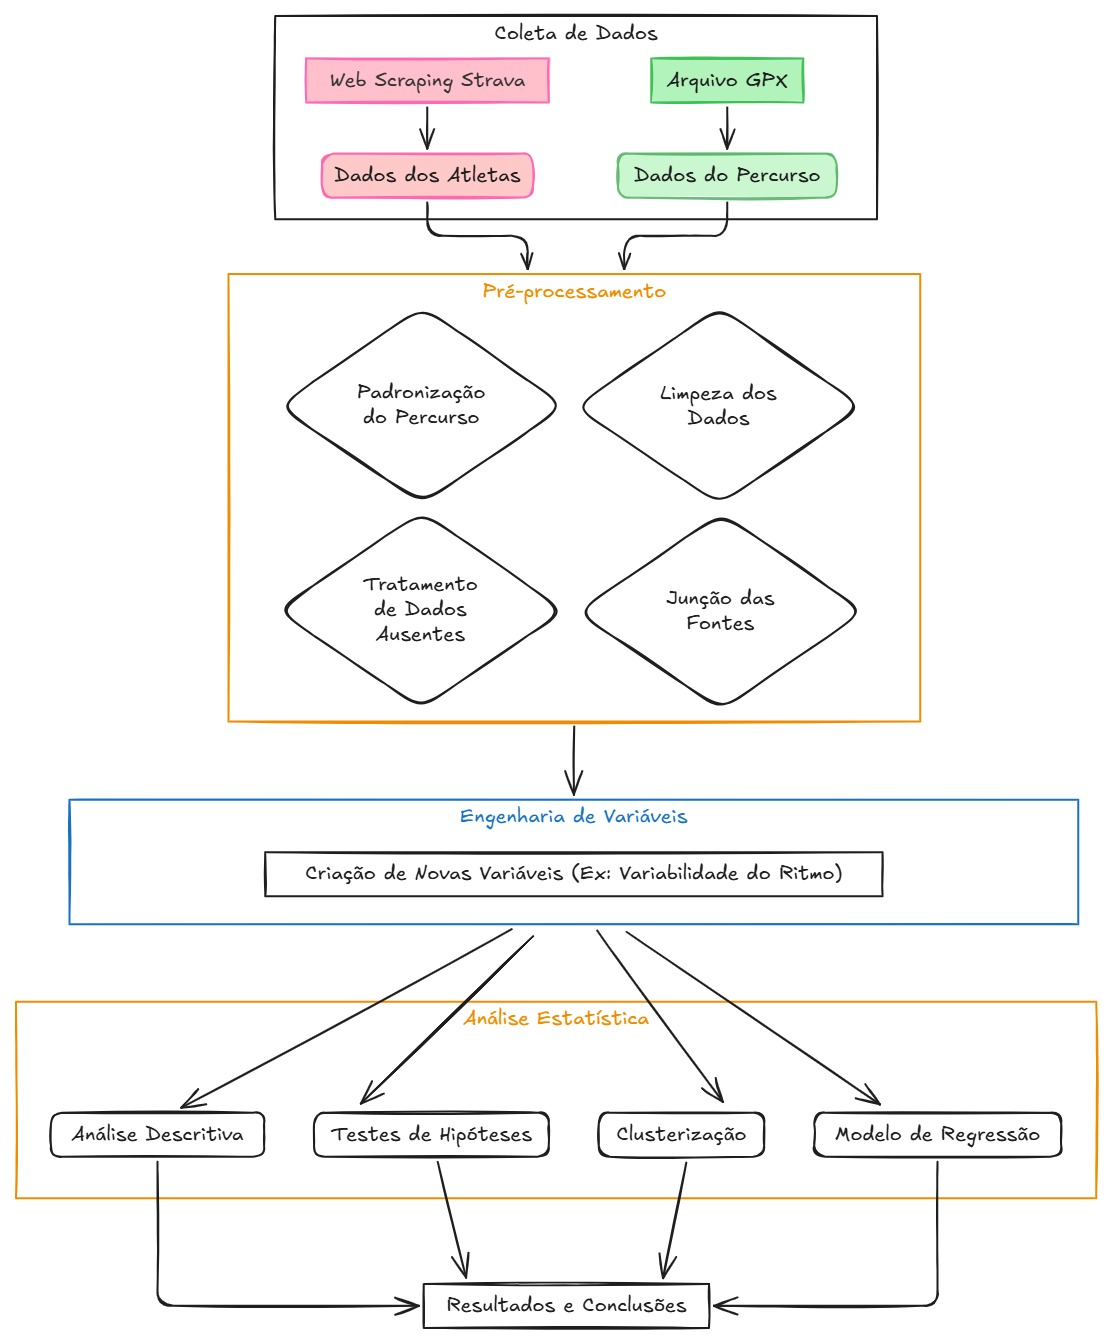
\includegraphics[width=0.75\textwidth]{Imagens/fluxo_trabalho.png}
    \caption{Fluxograma do processo de coleta e análise de dados. Fonte: Elaborado pelo autor (2025).}
    \label{fig:fluxograma}
\end{figure}

\section{Delineamento da Pesquisa}

Foi realizado um estudo quantitativo, de caráter descritivo e explicativo. Descritivo por meio da Análise Exploratória de Dados (AED), que visa caracterizar o perfil dos atletas da amostra. Explicativo ao utilizar técnicas de estatística inferencial, como a regressão linear múltipla, para modelar e explicar a relação entre um conjunto de variáveis e o desempenho final dos corredores.

\section{Fonte e Natureza dos Dados}
\label{sec:fonte_dados}

Os dados utilizados neste estudo foram extraídos da plataforma de rastreamento de atividades físicas Strava, referentes às edições de 2022 e 2023 da prova de \emph{trekking} de montanha \textit{La Misión Brasil}, na modalidade de 35 quilômetros. A extração foi realizada por meio de técnicas de \emph{web scraping}, conforme detalhado na Seção \ref{subsec:scraping}.

A natureza do conjunto de dados original era granular, com cada linha representando o desempenho de um único atleta em um quilômetro específico da prova. Essa estrutura, embora detalhada, não era adequada para uma análise centrada no desempenho geral do atleta, necessitando de uma etapa de agregação.

\section{Coleta e Pré-processamento dos Dados}

A obtenção dos dados foi dividida em quatro fases principais: padronização das informações do percurso, extração automatizada de dados da web, limpeza e estruturação final do conjunto de dados.

\subsection{Padronização dos Dados do Percurso via GPX}
\label{subsec:gpx}

A fim de garantir a consistência e a padronização das variáveis geográficas do percurso para todos os atletas, evitando discrepâncias inerentes a diferentes dispositivos de GPS, o ponto de partida foi a análise de um arquivo GPX (GPS Exchange Format) oficial da prova. Este arquivo foi processado para extrair informações de elevação a cada quilômetro, criando um gabarito do percurso com 36 segmentos. Essa abordagem permitiu que variáveis como ganho de elevação positivo e negativo de um determinado quilômetro fossem padronizadas e atribuídas de forma idêntica a todos os corredores da amostra.

\subsection{Extração de Dados via \textit{Web Scraping}}
\label{subsec:scraping}
Para a extração dos dados de desempenho e demográficos dos atletas, foi desenvolvida uma solução de \emph{web scraping} utilizando a linguagem de programação Python e a biblioteca \texttt{Selenium}, que permite a automação de navegadores web. O processo exigiu a autenticação em uma conta de usuário com assinatura paga na plataforma Strava para acessar os dados detalhados. O fluxo de extração foi estruturado da seguinte forma:

\begin{enumerate}
    \item \textbf{Coleta de Links:} O ponto de partida foram as páginas de resultados (tabelas de classificação) das edições de 2022 e 2023 da prova. O script navegou por estas páginas e coletou as URLs individuais de cada atividade de atleta registrada.
    
    \item \textbf{Extração de Dados de Performance:} Em um processo iterativo, o script acessava a URL de cada atleta. A prioridade era extrair a tabela de ``Voltas'' (\texttt{laps}), identificada pelo seletor CSS \texttt{'li[data-tracking-element="laps"] a'}, que continha os dados detalhados de tempo a cada quilômetro. Caso esta tabela não estivesse disponível, o script adotava uma abordagem de \emph{fallback}, extraindo os dados da tabela de segmentos principal.
    
    \item \textbf{Extração de Dados Demográficos:} Para obter as variáveis de sexo, faixa etária e faixa de peso, foi empregada uma técnica de filtragem na página principal de resultados. O script aplicava sequencialmente cada filtro (ex: sexo masculino), extraía a lista de nomes dos atletas correspondentes e armazenava essa informação. Posteriormente, esses dados foram unificados com os dados de performance através do nome dos atletas.
    
    \item \textbf{Gestão de Desafios Técnicos:} Durante a execução, foi observado que a plataforma poderia apresentar lentidão no carregamento de elementos. Para contornar essa questão, pausas estratégicas de 5 segundos (\texttt{time.sleep(5)}) foram inseridas no código para garantir que as páginas estivessem completamente carregadas antes da extração, aumentando a robustez do processo.
\end{enumerate}
Importante ressaltar que a coleta foi restrita a dados de perfis e atividades publicamente compartilhados pelos usuários.

\begin{figure}[H]
    \centering
    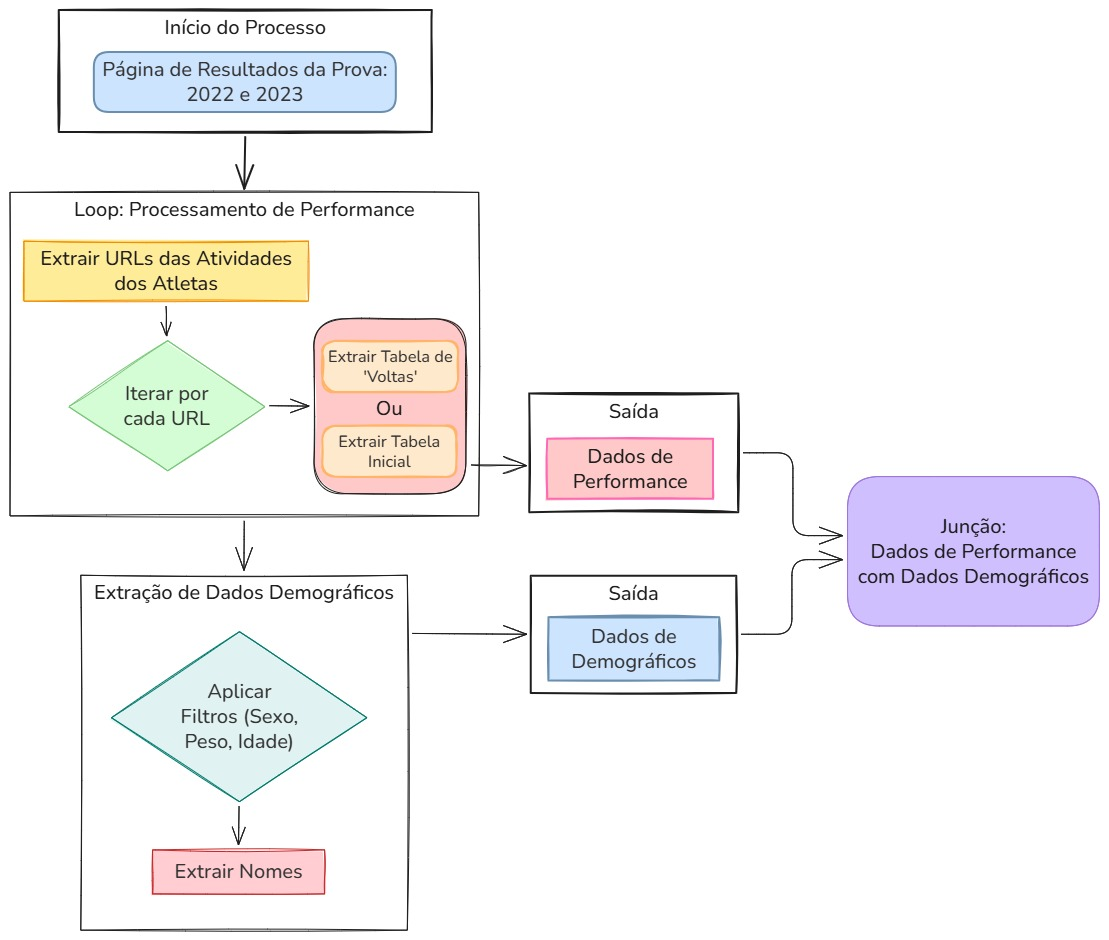
\includegraphics[width=0.7\textwidth]{Imagens/fluxo_webscraping.png}
    \caption{Fluxograma do processo de Web Scraping.}
    \label{fig:fluxograma_scraping}
    \caption*{Fonte: Elaborado pelo autor (2025).}
\end{figure}

\subsection{Limpeza e Estruturação dos Dados}
\label{subsec:limpeza}

Após a extração, foi realizado um rigoroso processo de limpeza e estruturação:
\begin{enumerate}
    \item \textbf{Unificação e Junção:} Os dados de performance dos atletas foram unidos (\emph{join}) aos dados padronizados do percurso (obtidos via GPX) pela coluna indicativa do quilômetro.
    
    \item \textbf{Tratamento de Duplicatas:} Identificou-se que 7 atletas participaram das duas edições da prova. Para garantir a independência das observações, foi mantida apenas a primeira participação de cada um, resultando em 166 atletas únicos nesta fase.
    
    \item \textbf{Padronização de Variáveis:} As colunas de `Tempo` e `Ritmo`, que se apresentavam em formatos distintos, foram unificadas e convertidas para uma unidade padrão de segundos.
    
    \item \textbf{Tratamento de Valores Ausentes:} A estratégia de tratamento de dados faltantes foi definida conforme a variável:
    \begin{itemize}
        \item \textbf{Frequência Cardíaca:} Dada a alta proporção de valores ausentes (superior a 70\%), indicando que a maioria dos atletas não utilizou ou não compartilhou dados de um monitor cardíaco, a variável foi removida do conjunto de dados para evitar a introdução de viés por meio de imputações complexas e pouco confiáveis.
        \item \textbf{Faixa de Peso:} Com aproximadamente 12,44\% de ausência, optou-se por tratar a ausência como uma informação em si. Foi criada a categoria ``Não Informado'', permitindo que o modelo analise se a própria decisão de não informar o peso está associada ao desempenho.
        \item \textbf{Sexo e Faixa Etária:} Com percentuais de ausência baixos (inferiores a 10\%), aplicou-se a técnica de exclusão \textit{listwise}. Esta abordagem foi considerada apropriada sob a suposição de que os dados eram ausentes completamente ao acaso (MCAR, \textit{Missing Completely at Random}), e que a remoção de um pequeno número de observações não introduziria um viés significativo na amostra final \citep[para uma discussão, ver][]{rubin1976}.
    \end{itemize}
\end{enumerate}
Ao final deste processo, consolidou-se um conjunto de dados final, limpo e estruturado no formato \emph{long}, contendo 109 atletas e 36 observações (quilômetros) para cada um.

\subsection{Agregação dos Dados}
\label{sec:preprocessamento}

Para transformar os dados granulares em um formato analítico focado no atleta, foi realizado um processo de agregação. Utilizando uma operação de agrupamento (\texttt{groupby}) por identificador de atleta, o conjunto de dados foi consolidado, passando de uma estrutura por quilômetro para uma estrutura em que cada linha representava um único atleta. Nesta etapa, foram criadas as variáveis agregadas fundamentais para a análise:
\begin{itemize}
    \item \textbf{\texttt{Tempo\_Final\_seg}:} Variável dependente principal do estudo, calculada como a soma total do tempo de cada quilômetro percorrido pelo atleta.
    \item \textbf{\texttt{Ritmo\_Medio\_seg}:} A média do tempo, em segundos, por quilômetro.
    \item \textbf{\texttt{Variabilidade\_Ritmo\_std}:} O desvio padrão do tempo por quilômetro, servindo como a principal métrica de consistência do ritmo do atleta ao longo da prova.
\end{itemize}

\section{Engenharia de Variáveis}
\label{sec:engenharia_variaveis_final}

Após feita a coleta de dados, assim como seu tratamento, foi realizado a etapa crucial da análise que consistiu na elaboração de novas métricas para capturar nuances da estratégia de prova e da performance dos atletas em diferentes terrenos. 

\subsection{Variáveis de Estratégia de Prova (\textit{Splits})}

Para analisar a distribuição de esforço, a prova foi dividida em duas metades: "Primeira Metade" (quilômetros 1-18) e "Segunda Metade" (quilômetros 19-36). A partir dessa segmentação, foram criadas as variáveis \texttt{Ritmo\_Medio\_Primeira\_Metade} e \texttt{Ritmo\_Medio\_Segunda\_Metade}.

Para uma comparação mais robusta da variação de ritmo, foi criada a variável \texttt{diff\_relativa\_segunda\_primeira\_parte}. A justificativa para o uso de uma métrica relativa, em vez de uma diferença absoluta, reside no fato de que uma mesma variação de tempo (e.g., 30 segundos) possui significados distintos para um atleta de elite e um amador. A normalização pelo ritmo médio do próprio atleta gera uma medida de eficiência de \emph{pacing} mais justa e comparável entre corredores de diferentes níveis de habilidade.

\subsection{Variáveis Baseadas em Terreno (Altimetria)}

Para isolar o desempenho em diferentes inclinações, cada quilômetro do percurso foi classificado como "SUBIDA", "DESCIDA", "PLANO" ou "MISTO". Essa classificação foi realizada por uma função customizada (\texttt{Sob\_Desc}) baseada em regras sobre o desnível positivo e negativo de cada trecho. A partir dessa categorização, foram calculadas as variáveis de ritmo médio para cada tipo de terreno, como \texttt{Ritmo\_Medio\_SUBIDA} e \texttt{Ritmo\_Medio\_DESCIDA}.

\subsection{Índices de Performance Relativa}

Visando quantificar a especialização técnica dos atletas, foram desenvolvidos índices normalizados que comparam o desempenho em terrenos específicos com o desempenho geral do próprio indivíduo.
\begin{itemize}
    \item \textbf{\texttt{indice\_subida}:} Mede o quão mais lento um atleta é na subida em comparação com sua própria média geral.
    \item \textbf{\texttt{indice\_descida}:} Mede o quão mais rápido um atleta é na descida em comparação com sua média geral.
    \item \textbf{\texttt{indice\_descida\_vs\_subida}:} Compara diretamente a performance nos dois terrenos-chave, servindo como uma métrica da capacidade de aceleração relativa do atleta em descidas versus subidas.
\end{itemize}

\section{Análise Estatística}
\label{sec:analise_estatistica}

A análise dos dados foi conduzida por meio de um conjunto de técnicas estatísticas, onde a escolha de cada teste foi rigorosamente justificada pelos pressupostos dos dados.

\subsection{Análise Descritiva}
Inicialmente, foi realizada uma análise descritiva com o uso de medidas de tendência central (média, mediana) e dispersão (desvio padrão) para as variáveis quantitativas, e distribuições de frequência para as variáveis categóricas. Visualizações gráficas como histogramas, diagramas de dispersão e \emph{boxplots} foram utilizadas para compreensão visual dos dados e distribuição das variáveis.

\subsection{Testes de Hipóteses}

A comparação do tempo final entre diferentes grupos demográficos foi realizada por meio de testes de hipóteses não-paramétricos. A escolha por essa abordagem foi motivada pela rejeição da hipótese de normalidade da variável resposta \texttt{Tempo\_Final\_seg} nos subgrupos, verificada pelo teste de Shapiro-Wilk para um nível de significância $\alpha = 0.05$. A estatística não-paramétrica é robusta a distribuições não-normais, baseando-se nos postos (\textit{ranks}) das observações em vez de seus valores absolutos \citep{siegel1988}.

\begin{itemize}
    \item \textbf{Comparação entre Sexos:} Para comparar a distribuição do tempo final entre homens e mulheres, utilizou-se o teste de Mann-Whitney U. As hipóteses testadas foram:
    \begin{itemize}
        \item $H_0$: A distribuição do tempo final é a mesma para ambos os sexos.
        \item $H_a$: A distribuição do tempo final é diferente entre os sexos.
    \end{itemize}
    
    \item \textbf{Comparação entre Faixas Etárias e de Peso:} Para comparar o tempo final entre três ou mais grupos independentes (faixas etárias e faixas de peso), empregou-se o teste de Kruskal-Wallis. As hipóteses foram:
    \begin{itemize}
        \item $H_0$: As distribuições do tempo final são as mesmas em todas as faixas (etárias ou de peso).
        \item $H_a$: Pelo menos uma faixa possui uma distribuição de tempo final diferente das demais.
    \end{itemize}
    Em caso de rejeição da hipótese nula, foi aplicado o teste \textit{post-hoc} de Dunn com a correção de Bonferroni para identificar quais pares de grupos apresentavam diferenças estatisticamente significativas, controlando a taxa de erro do Tipo I que inflaciona com múltiplas comparações.
\end{itemize}

\subsection{Análise de Associação}
Para investigar a relação entre a performance (\texttt{Tempo\_Final\_seg}) e a consistência do ritmo (\texttt{Variabilidade\_Ritmo\_std}), utilizou-se o coeficiente de correlação de postos de Spearman ($\rho$). Este método foi escolhido em detrimento da correlação de Pearson devido à não-normalidade das variáveis. Conforme definem \citet{siegel1988}, o teste de Spearman avalia a força e a direção de uma relação monotônica (não necessariamente linear) entre duas variáveis. As hipóteses testadas foram:
\begin{itemize}
    \item $H_0: \rho = 0$ (Não há associação monotônica entre as variáveis).
    \item $H_a: \rho \neq 0$ (Existe uma associação monotônica entre as variáveis).
\end{itemize}

\subsection{Análise de Agrupamento}

Com o objetivo de identificar perfis distintos de corredores ("personas") com base em suas características de prova, foi aplicada a técnica de clusterização não-supervisionada K-Means. O propósito desta análise foi segmentar a amostra em grupos intrinsecamente homogêneos e extrinsecamente heterogêneos, revelando diferentes estratégias e especialidades de desempenho dos atletas.

\subsubsection{Pré-processamento das Variáveis para Clusterização}

O algoritmo K-Means agrupa os dados minimizando a variância intra-cluster, um processo que se baseia fundamentalmente no cálculo de distâncias (tipicamente a distância Euclidiana) entre as observações e os centróides dos clusters. Quando as variáveis de entrada (features) possuem escalas e magnitudes muito diferentes — como, por exemplo, uma variável de tempo em segundos (na casa dos milhares) e um índice de performance (na casa de 0.1 a 0.3) — o cálculo da distância pode ser enviesado. A variável com a maior magnitude iria dominar o cálculo, minimizando ou até anulando a contribuição das outras variáveis para a definição dos grupos.\citep{muller2016}.

Para suavizar este efeito e garantir que todas as variáveis tivessem a mesma importância relativa no processo de agrupamento, foi realizado um pré-processamento de padronização dos dados por meio da técnica \textit{StandardScaler}. Este método transforma cada variável para que ela passe a ter uma média igual a zero e um desvio padrão igual a um. A escolha por essa técnica se justifica pois muitos algoritmos de aprendizado de máquina assumem que as características estão centradas em zero e possuem variância na mesma ordem, evitando que uma variável domine a função objetivo do algoritmo \citep{scikitlearn_preprocessing}. A fórmula para a padronização de cada observação (x) em uma variável é dada por:

\begin{equation}
    z = \frac{x - \mu}{\sigma}
    \label{eq:standardscaler}
\end{equation}

Onde:
\begin{itemize}
    \item $z$ é o valor padronizado (ou z-score);
    \item $x$ é o valor original da observação;
    \item $\mu$ é a média de todos os valores da variável (feature);
    \item $\sigma$ é o desvio padrão de todos os valores da variável.
\end{itemize}

Este passo metodológico foi crucial para assegurar que a formação dos clusters fosse resultado dos padrões nos dados, e não de uma distorção causada pelas diferentes escalas das métricas de desempenho.

\subsubsection{Seleção do Número de Clusters (k)}

A determinação do número ideal de agrupamentos ($k$) é um parâmetro fundamental para o algoritmo K-Means. Para esta finalidade, foi empregado o Método do Cotovelo (\textit{Elbow Method})\citep{thorndike1953}. Este método consiste em executar o algoritmo de clusterização para um intervalo de valores de $k$ (e.g., de 1 a 10) e calcular a soma dos quadrados das distâncias intra-cluster (inércia) para cada valor. O número ótimo de clusters é visualmente identificado no ponto do gráfico onde a adição de um novo cluster não resulta em uma diminuição significativa da inércia, formando um "cotovelo" na curva.


\subsection{Modelagem Preditiva}
Para modelar a relação entre o tempo final e as diversas métricas de desempenho e demográficas, foi ajustado um modelo de Regressão Linear Múltipla, utilizando o método de Estimação por Mínimos Quadrados Ordinários (OLS).

\subsubsection{Especificação do Modelo}
O modelo teórico assume a seguinte forma:
$$ Y = \beta_0 + \beta_1 X_1 + \beta_2 X_2 + \dots + \beta_p X_p + \epsilon $$
Onde $Y$ é a variável dependente (\texttt{Tempo\_Final\_seg}), $X_1, \dots, X_p$ são as variáveis preditoras, $\beta_0, \dots, \beta_p$ são os coeficientes a serem estimados, e $\epsilon$ é o termo de erro aleatório, que se assume seguir uma distribuição normal com média zero e variância constante ($\epsilon \sim N(0, \sigma^2)$).

\subsubsection{Pressupostos do Modelo}
A validade das inferências do modelo OLS depende de um conjunto de pressupostos sobre os erros \citep{montgomery2012}:
\begin{enumerate}
    \item \textbf{Linearidade:} A relação entre as variáveis preditoras e a variável resposta é linear.
    \item \textbf{Independência dos Erros:} Os erros $\epsilon_i$ são independentes entre si.
    \item \textbf{Homocedasticidade:} Os erros possuem variância constante ($\text{Var}(\epsilon_i) = \sigma^2$) para todos os níveis das variáveis preditoras.
    \item \textbf{Normalidade dos Erros:} Os erros são normalmente distribuídos.
\end{enumerate}
A verificação destes pressupostos foi realizada a posteriori, por meio da análise gráfica dos resíduos do modelo ajustado.

\subsubsection{Seleção de Variáveis e Avaliação do Modelo}
Partindo de um modelo inicial com todas as variáveis preditoras potenciais, foi aplicado um processo de seleção de variáveis \textit{backward elimination}. A cada passo, a variável com o maior p-valor acima do nível de significância de 0.05 era removida, buscando-se um modelo final que fosse parcimonioso e interpretável.

Para evitar problemas de multicolinearidade (alta correlação entre preditores), o Fator de Inflação de Variância (VIF) foi calculado para as variáveis do modelo final. Um VIF superior a 5 foi considerado como indicativo de multicolinearidade problemática, levando à remoção da variável em questão.

A qualidade do ajuste do modelo final foi avaliada pelo coeficiente de determinação ajustado ($R^2_{\text{adj}}$), pela significância estatística global do modelo (teste F) e dos coeficientes individuais (teste t), e pela análise de resíduos para validação dos pressupostos.


\section{Softwares Utilizados}

Todas as etapas de coleta, tratamento e análise estatística dos dados foram conduzidas na linguagem de programação Python (versão >= 3.11), com o auxílio de bibliotecas consagradas para manipulação e análise de dados, como Pandas, NumPy, Matplotlib, Seaborn, e para modelagem estatística, como Scikit-learn e Statsmodels.

% --- FIM DO CAPÍTULO DE METODOLOGIA ---

    %====================================================================
    % Resultados Preliminares
    %====================================================================
    \newpage
    \chapter{Resultados}
\label{chap:resultados}

Este capítulo apresenta os resultados obtidos a partir da aplicação da metodologia descrita anteriormente. A análise está estruturada de forma a construir uma compreensão progressiva dos fatores que influenciam o desempenho dos atletas na prova, partindo de uma análise descritiva geral, passando pela investigação de fatores demográficos e de estratégia, pela identificação de perfis de corredores e, finalmente, culminando na construção de um modelo preditivo.

\section{Análise Descritiva da Amostra}

Após os procedimentos de limpeza, tratamento e agregação dos dados, a amostra final consolidada para análise foi composta por 109 atletas únicos. A variável resposta principal do estudo, o tempo final de prova (\texttt{Tempo\_Final\_min}), apresentou uma considerável variabilidade, como detalhado na Tabela \ref{tab:descritiva_geral} e ilustrado na Figura \ref{fig:dist_tempo_final}.

% --- Tabela Descritiva Geral ---
\begin{table}[]
\centering
\caption{Estatísticas descritivas das principais variáveis de desempenho (N=109).}
\label{tab:descritiva_geral}
\resizebox{\columnwidth}{!}{%
\begin{tabular}{@{}lccc@{}}
\toprule
\textbf{Estatística} & \textbf{Tempo Final (min)} & \textbf{Ritmo Médio (min/km)} & \multicolumn{1}{l}{\textbf{Variabilidade do Ritmo (min)}} \\ \midrule
Média                & 422.00                     & 11.87                         & 7.02                                                      \\
Desvio Padrão        & 122.97                     & 3.50                          & 3.26                                                      \\
Mínimo               & 236.40                     & 6.57                          & 2.90                                                      \\
Mediana              & 389.82                     & 10.82                         & 5.65                                                      \\
Máximo               & 790.93                     & 22.60                         & 16.51                                                     \\ \bottomrule
\end{tabular}%
}
\end{table}
\begin{flushleft}
    \footnotesize Fonte: Elaborado pelo autor (2025).
\end{flushleft}

O tempo médio para completar a prova foi de 422 minutos (aproximadamente 7 horas), com uma grande dispersão nos resultados (desvio padrão de 123 minutos). O atleta mais rápido completou o percurso em 236 minutos (menos de 4 horas), enquanto o último concluinte levou 791 minutos (mais de 13 horas). A Figura \ref{fig:dist_tempo_final} mostra a distribuição dos tempos, que apresenta uma leve assimetria à direita.

% --- Figura Distribuição do Tempo Final ---
\begin{figure}[H]
    \centering
    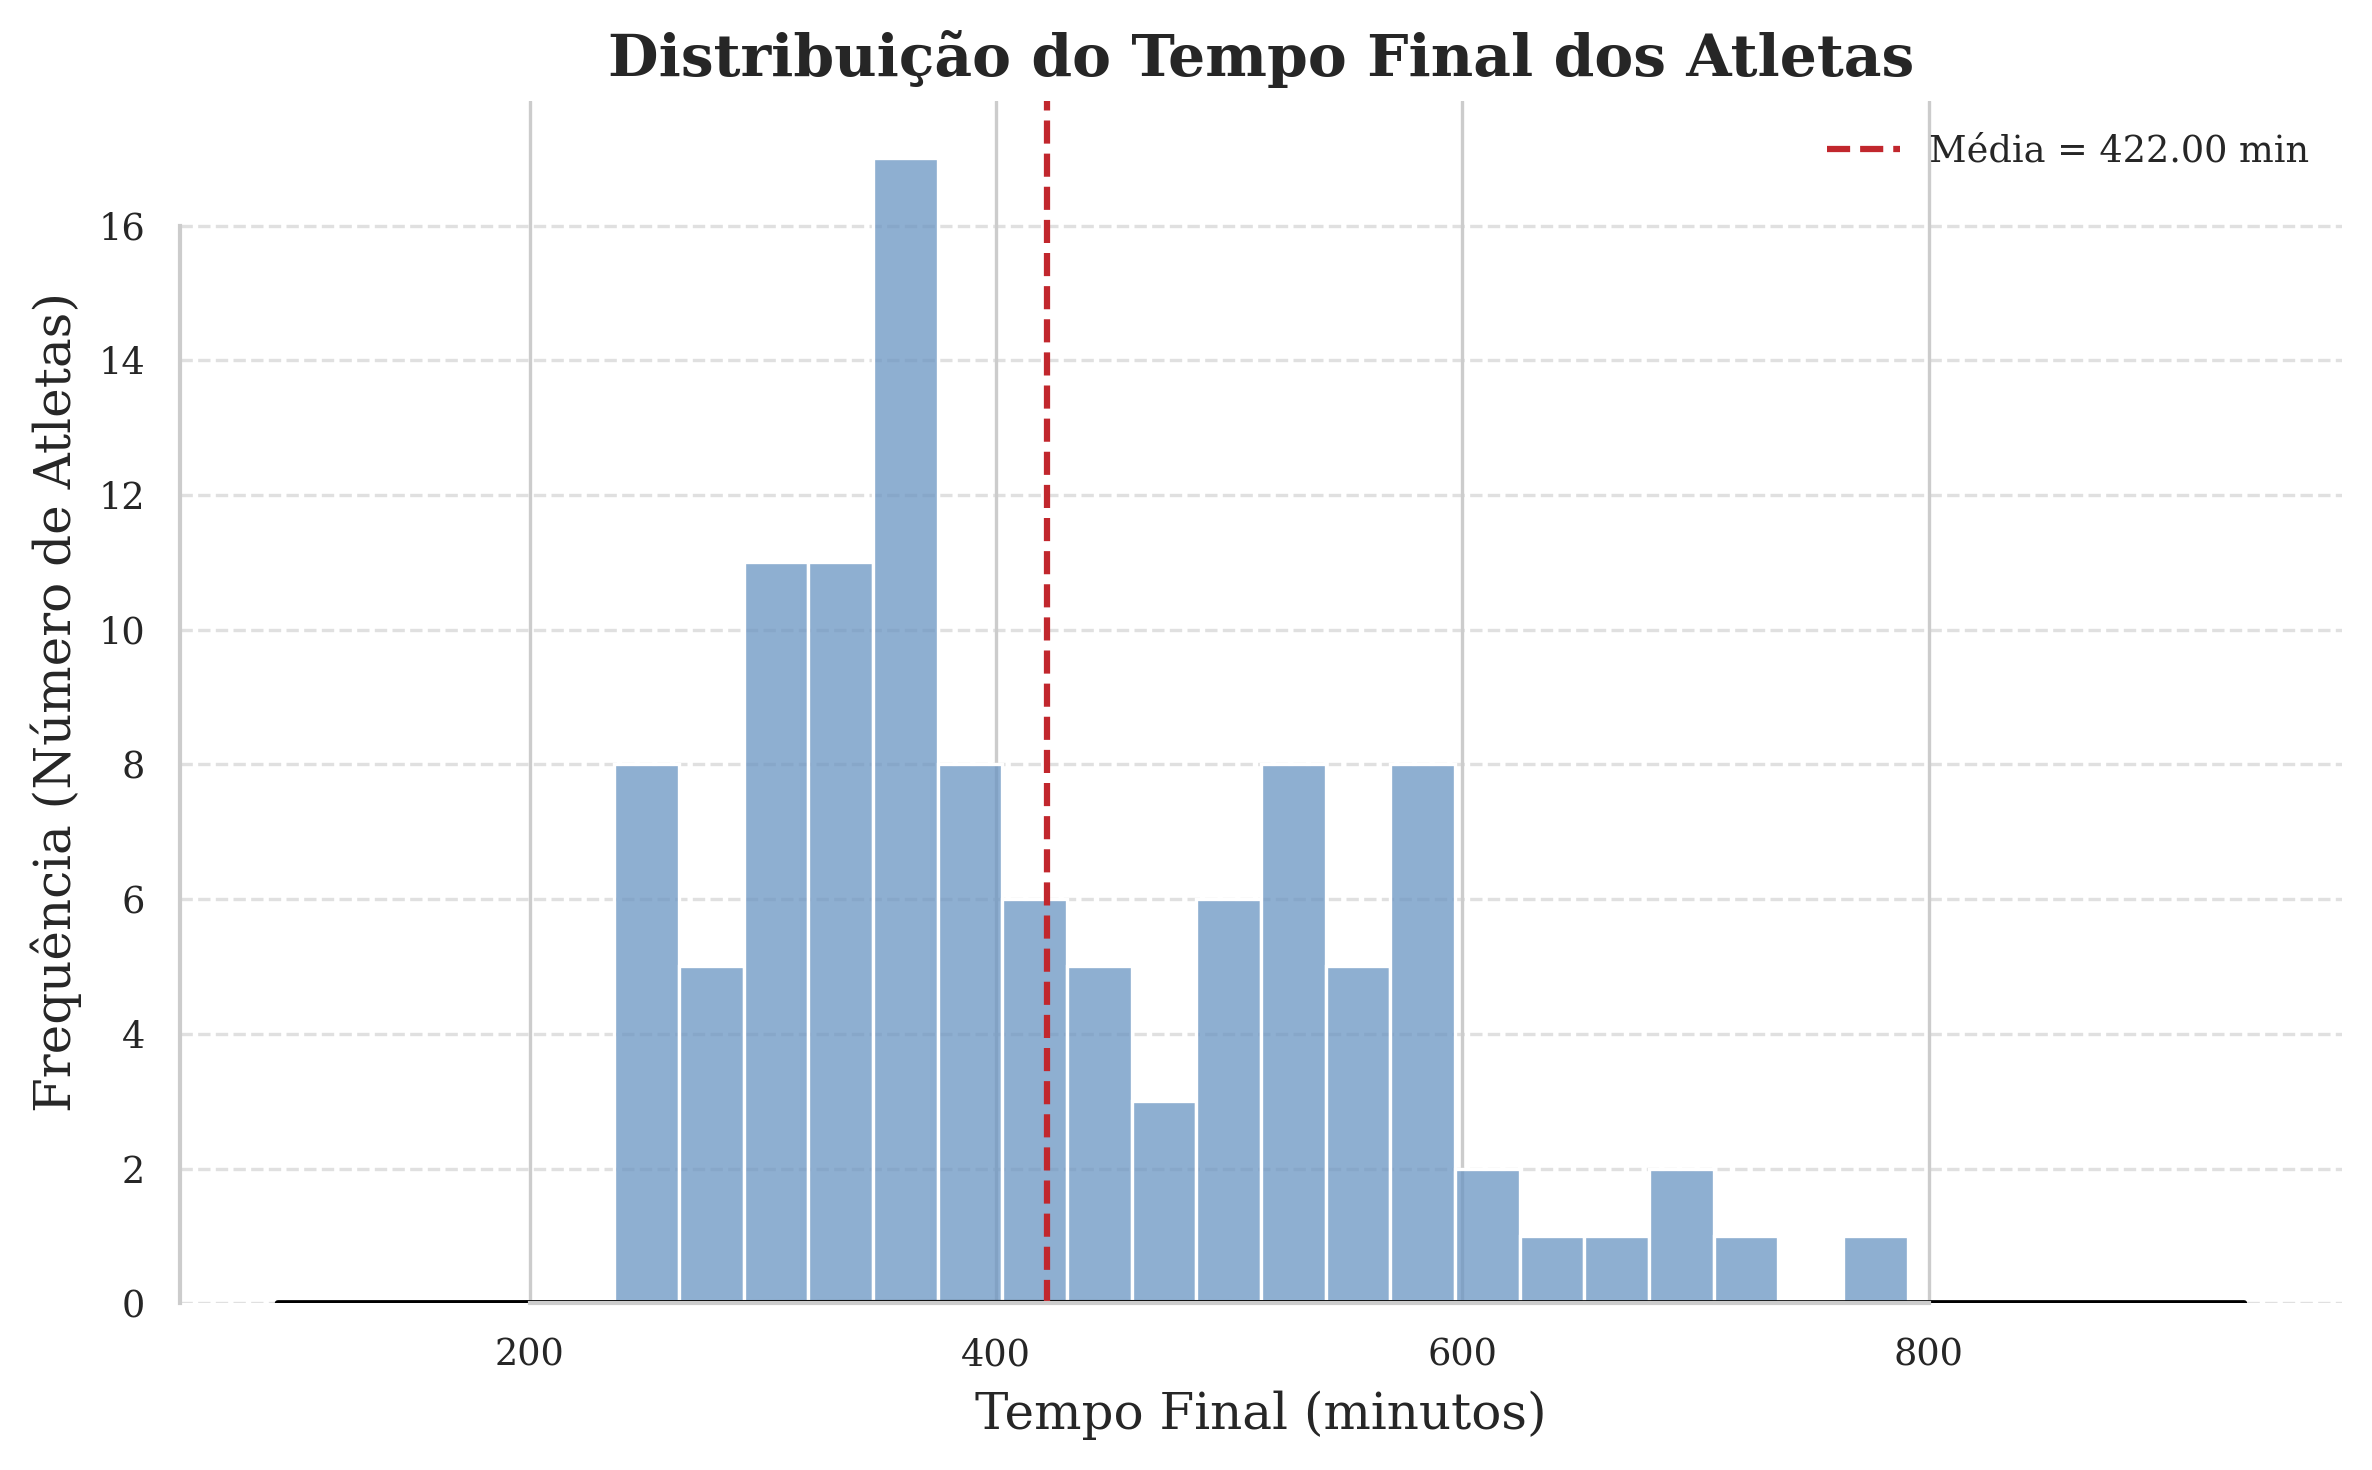
\includegraphics[width=0.8\textwidth]{Imagens/distribuicao_tempo_final.png}
    \caption{Histograma da distribuição do Tempo Final em minutos.}
    \label{fig:dist_tempo_final}
    \caption*{Fonte: Elaborado pelo autor (2025).}
\end{figure}

\section{Análise de Fatores Demográficos}

Nesta seção, investiga-se a relação entre o desempenho e as características demográficas dos atletas: sexo, faixa etária e peso.

\subsection{Influência do Sexo no Desempenho}

A amostra foi composta por 78 homens e 31 mulheres. A análise comparativa revelou uma diferença estatisticamente significativa entre os grupos. O teste de Shapiro-Wilk indicou que a variável \texttt{Tempo\_Final\_min} não seguia uma distribuição normal para ambos os grupos (p=0.0008 para homens e p=0.0360 para mulheres), justificando o uso de um teste não-paramétrico.

O Teste de Mann-Whitney U resultou em um p-valor de \textbf{0.0319}, que, sendo inferior ao nível de significância $\alpha=0.05$, nos leva a rejeitar a hipótese nula. Conclui-se que existe uma diferença estatisticamente significativa no tempo de prova entre homens e mulheres. Conforme observado na Figura \ref{fig:boxplot_sexo} e na Tabela \ref{tab:descritiva_sexo}, os homens apresentaram, em média, um tempo de conclusão menor (média de 405.4 min) em comparação com as mulheres (média de 463.7 min).

% --- Figura Boxplot por Sexo ---
\begin{figure}[H]
    \centering
    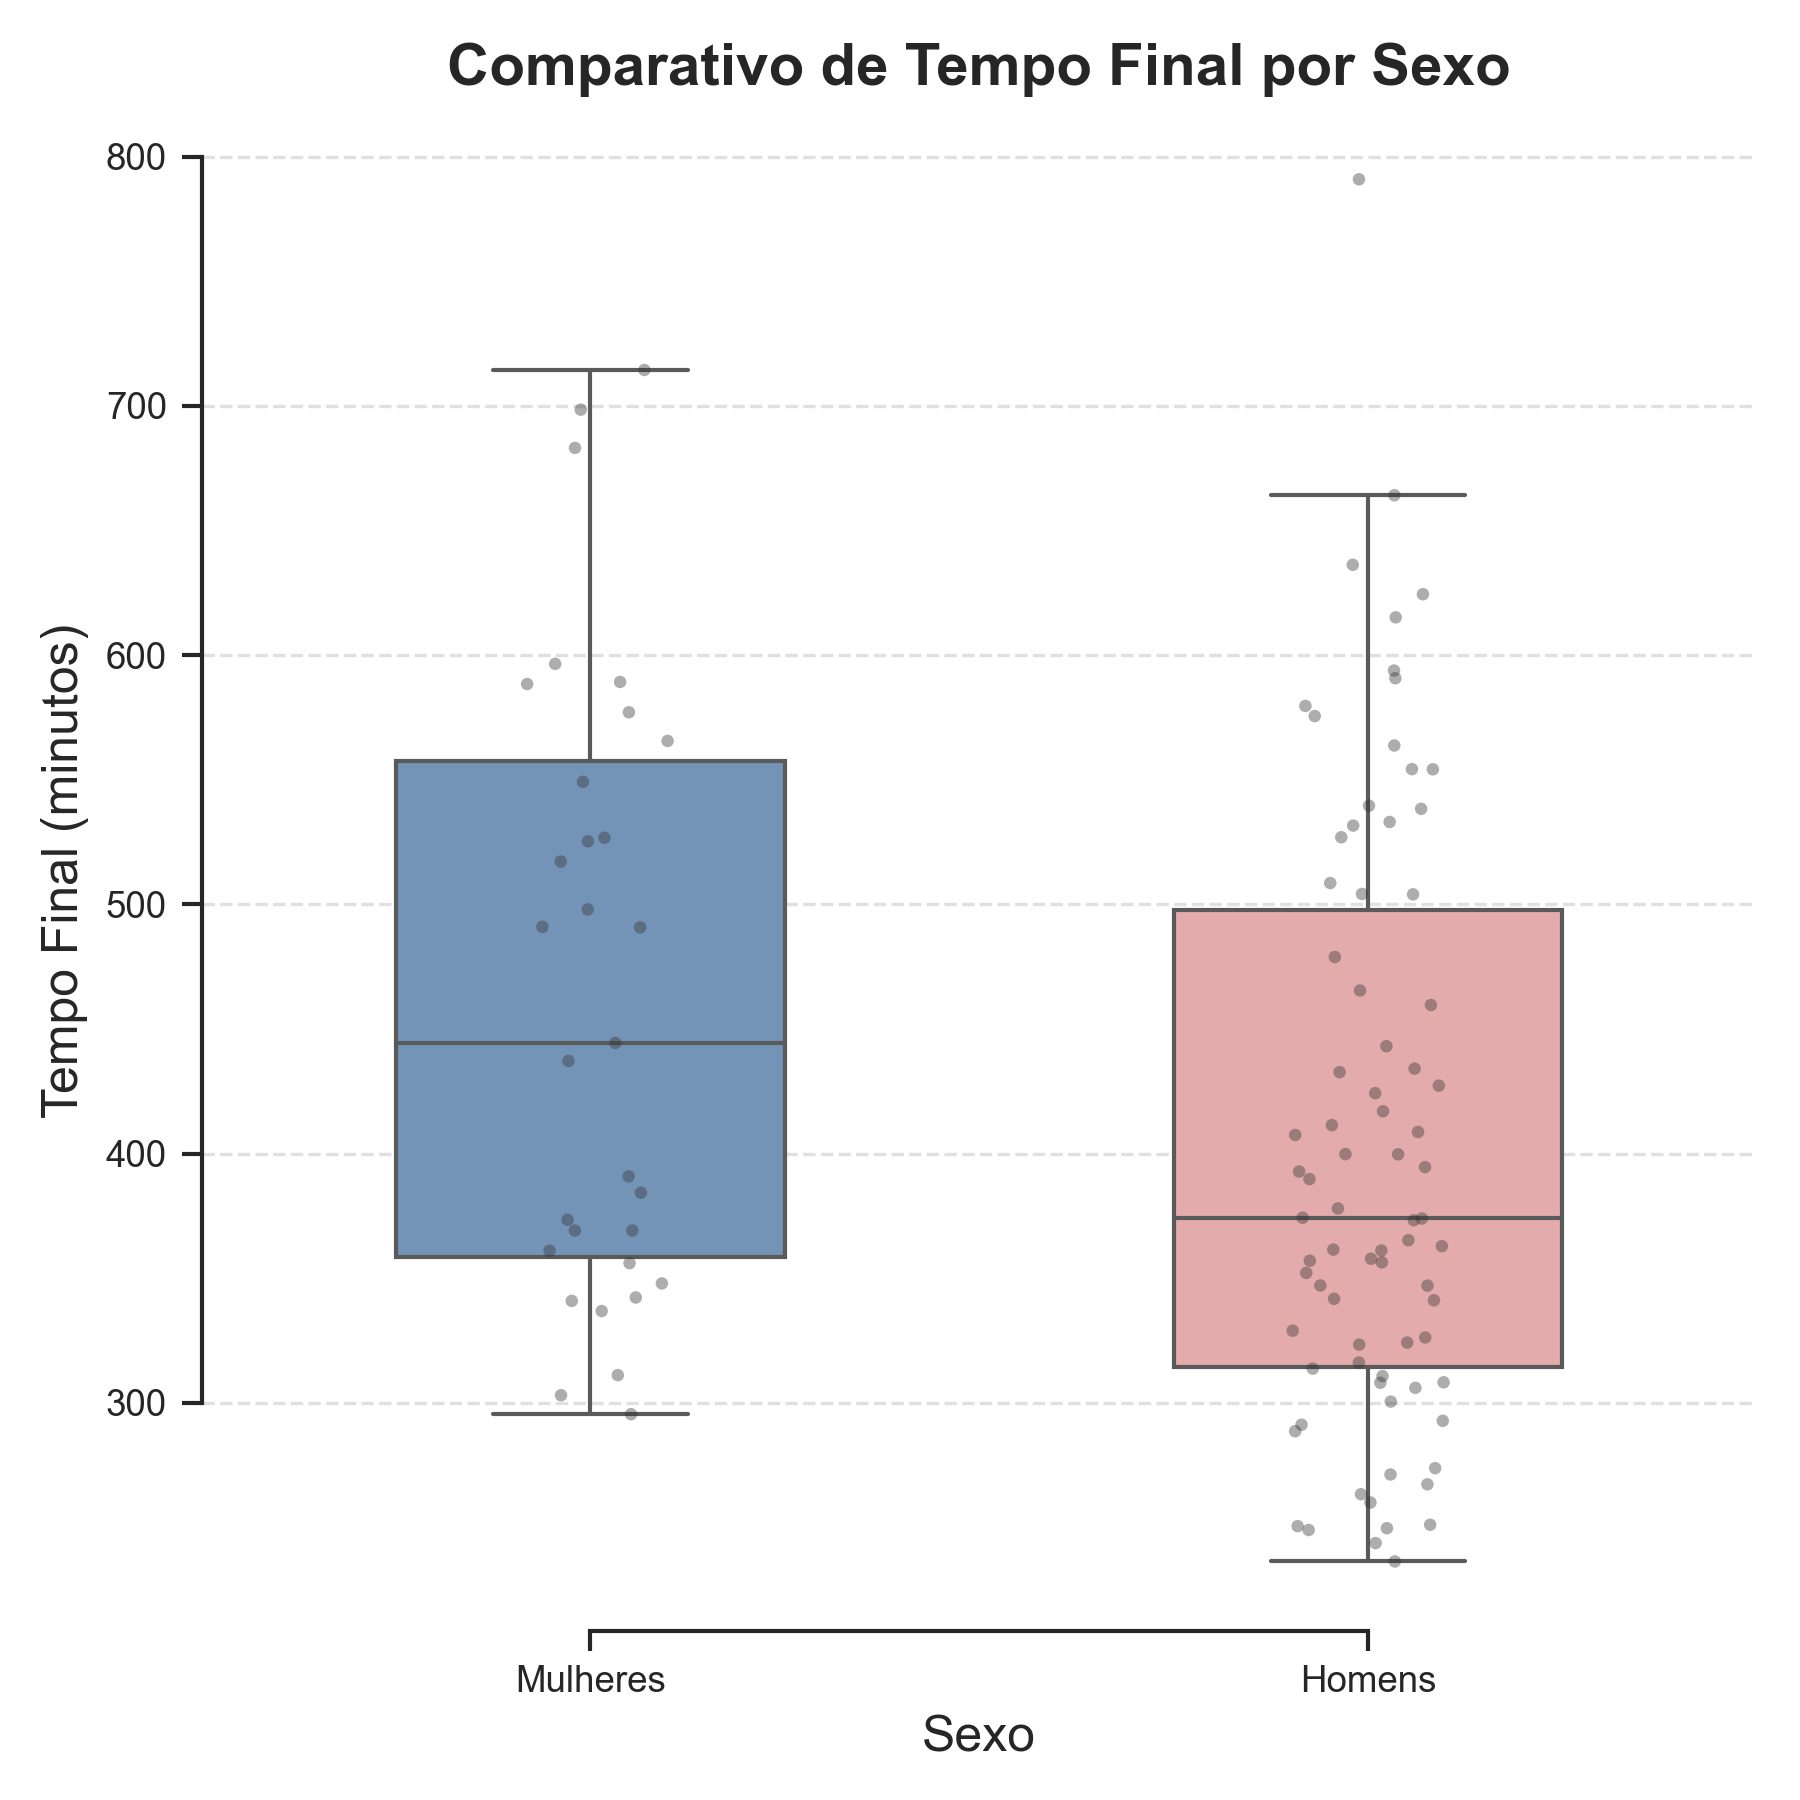
\includegraphics[width=0.8\textwidth]{Imagens/boxplot_tempo_por_sexo.png}
    \caption{Boxplot comparativo do Tempo Final por Sexo.}
    \label{fig:boxplot_sexo}
    \caption*{Fonte: Elaborado pelo autor (2025).}
\end{figure}

% --- Tabela Descritiva por Sexo ---
\begin{table}[H]
\centering
\caption{Estatísticas descritivas do Tempo Final (min) por Sexo.}
\label{tab:descritiva_sexo}
\begin{tabular}{lcc}
\toprule
\textbf{Estatística} & \textbf{Homens} & \textbf{Mulheres} \\
\midrule
Média   & 405.43 & 463.71 \\
Mediana & 374.14 & 444.42 \\
Desvio Padrão & 119.60 & 123.35 \\
N       & 78     & 31     \\
\bottomrule
\end{tabular}
\caption*{Fonte: Elaborado pelo autor (2025).}
\end{table}

\subsection{Influência da Faixa Etária no Desempenho}

Os atletas foram distribuídos em cinco faixas etárias, com maior concentração entre 25 e 44 anos (72\% da amostra). O teste de Shapiro-Wilk apontou que múltiplos grupos não seguiam a normalidade, indicando o Teste de Kruskal-Wallis como a ferramenta adequada. Devido à presença de grupos com amostras pequenas (n=4 e n=6), um Teste de Permutação foi realizado para garantir a robustez do p-valor, resultando em \textbf{p=0.0360}.

Este resultado significativo indica que existe diferença no tempo de prova entre pelo menos duas faixas etárias. Para identificar quais grupos diferem entre si, foi aplicado o teste \textit{post-hoc} de Dunn com correção de Bonferroni (Tabela \ref{tab:dunn_faixa_etaria}).

% --- Figura Boxplot por Faixa Etária ---
\begin{figure}[H]
    \centering
    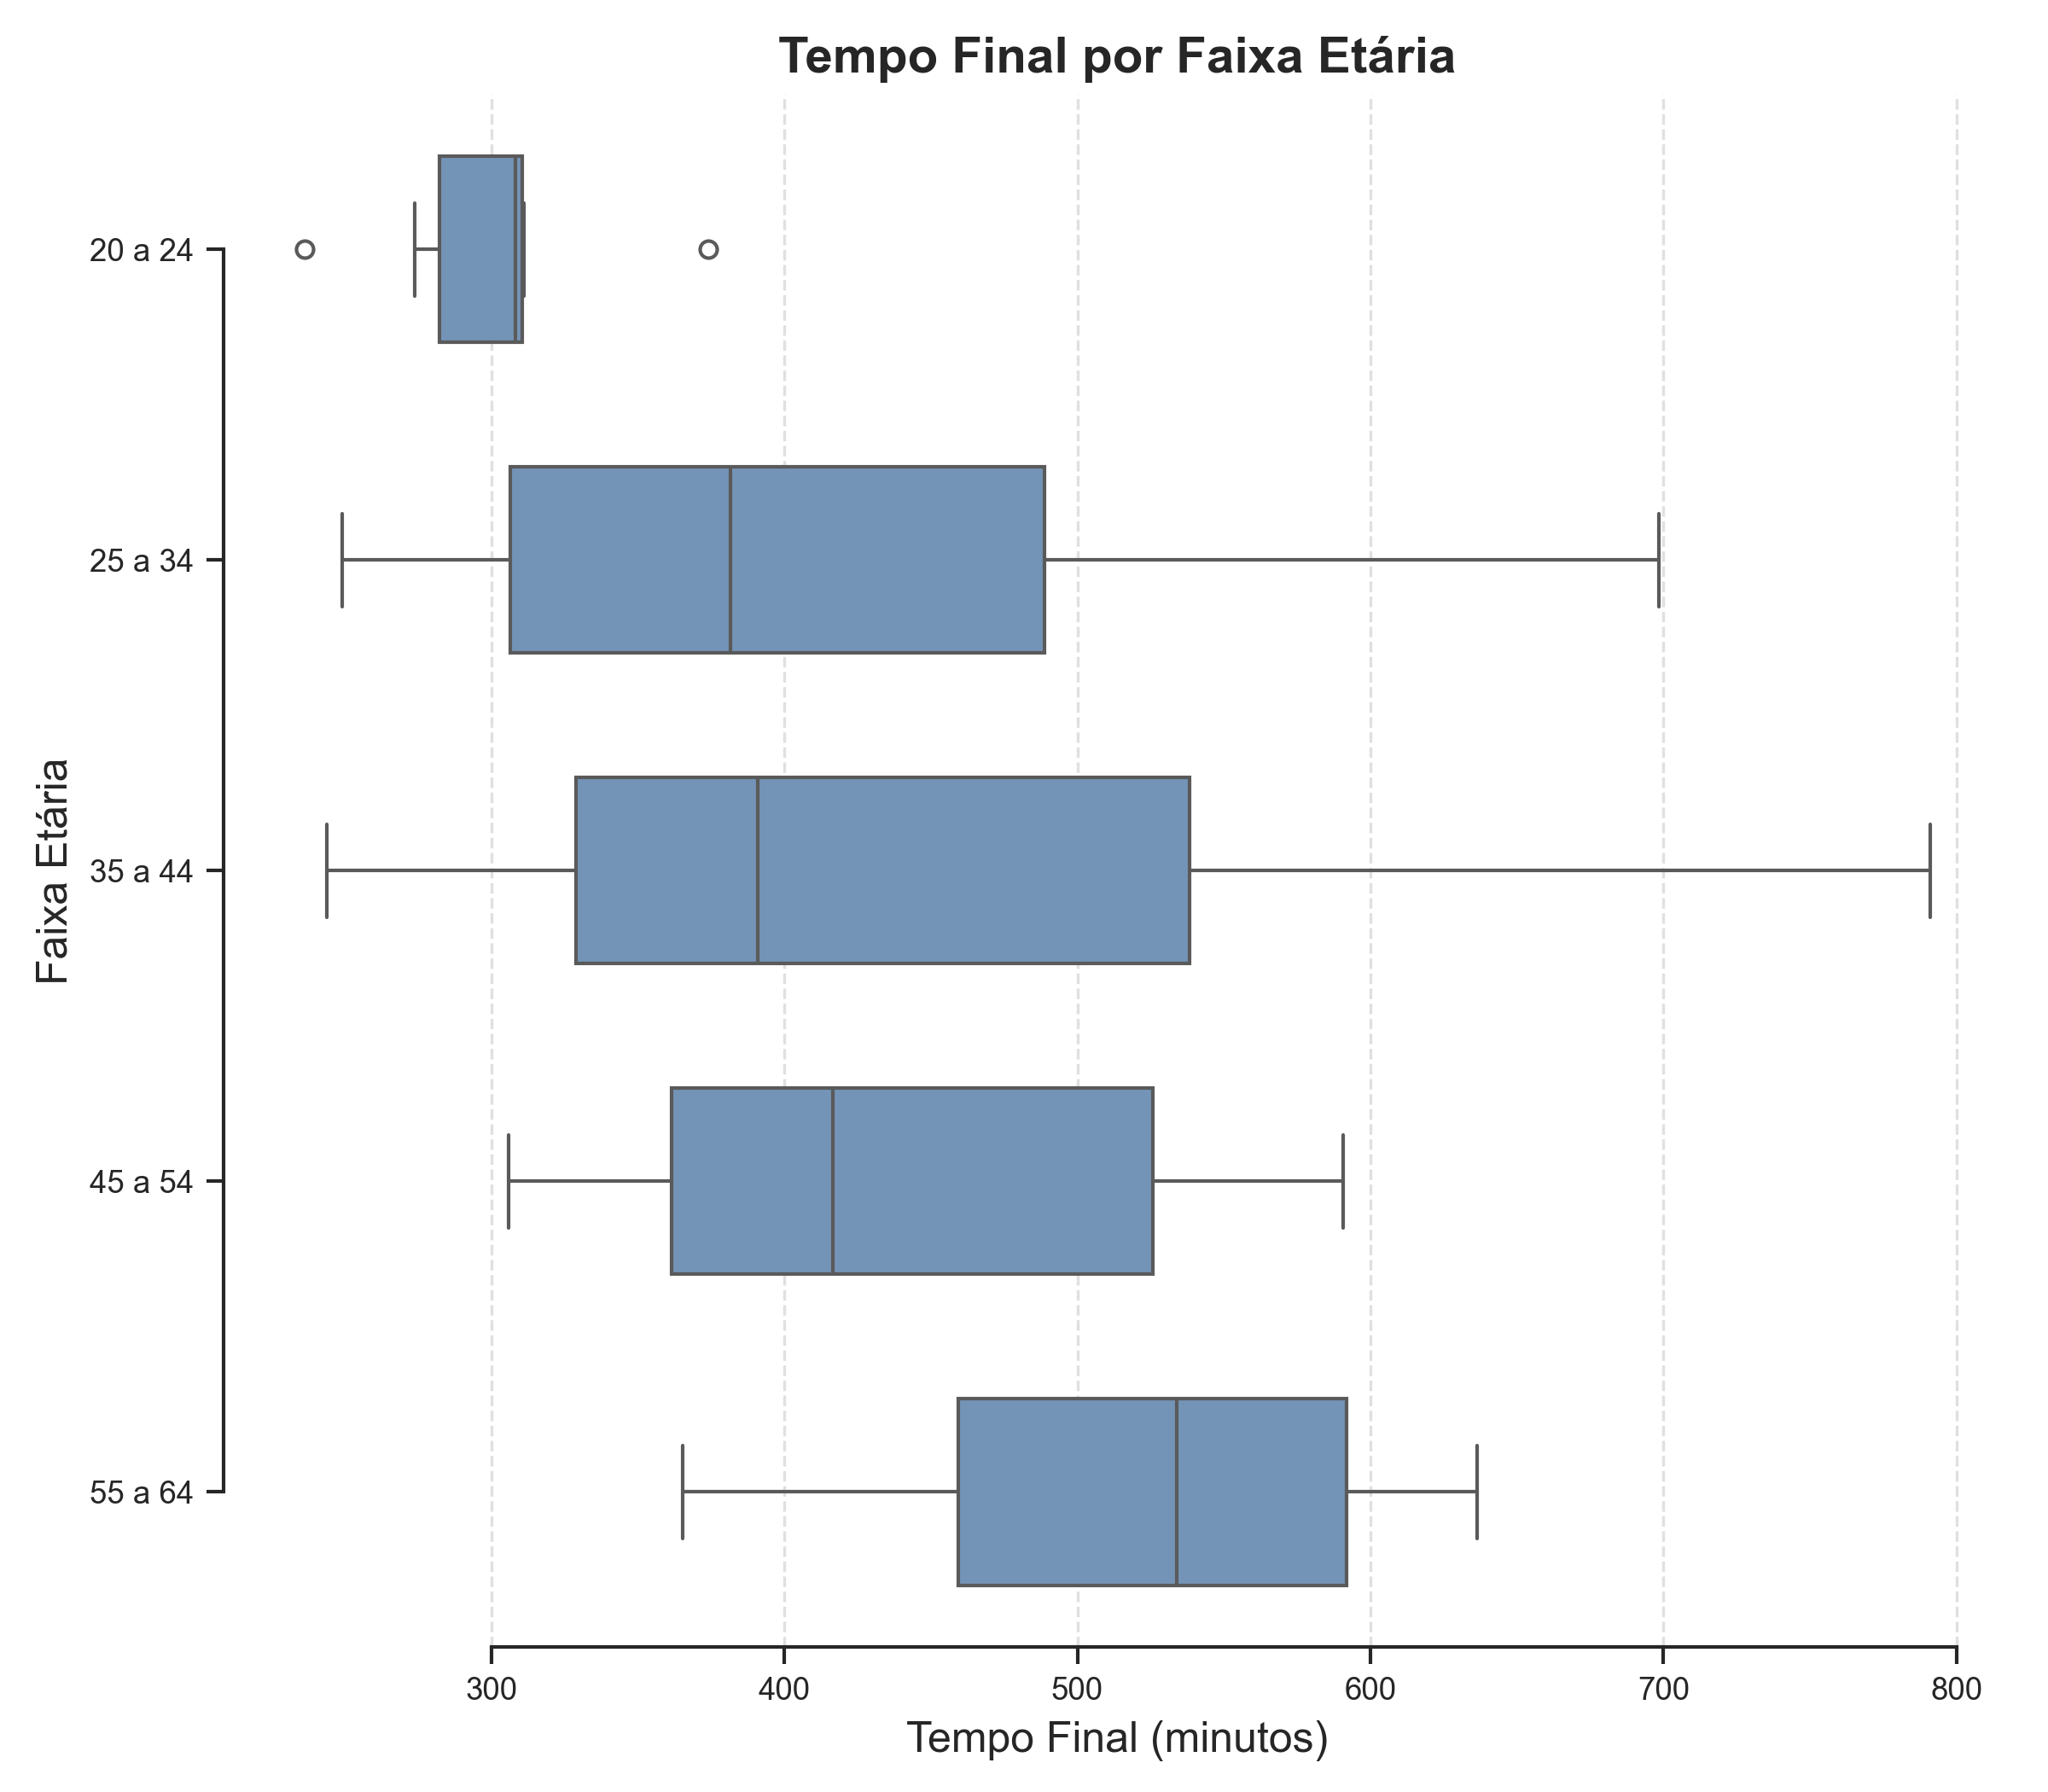
\includegraphics[width=0.8\textwidth]{Imagens/boxplot_tempo_por_faixa_etaria.png}
    \caption{Boxplot comparativo do Tempo Final por Faixa Etária.}
    \label{fig:boxplot_idade}
    \caption*{Fonte: Elaborado pelo autor (2025).}
\end{figure}

% --- Tabela Post-Hoc Dunn ---
\begin{table}[H]
\centering
\caption{Matriz de p-valores do teste \textit{post-hoc} de Dunn com correção de Bonferroni.}
\label{tab:dunn_faixa_etaria}
\begin{tabular}{lccccc}
\toprule
 & \textbf{20 a 24} & \textbf{25 a 34} & \textbf{35 a 44} & \textbf{45 a 54} & \textbf{55 a 64} \\
\midrule
\textbf{20 a 24} & 1.000 & - & - & - & - \\
\textbf{25 a 34} & 0.313 & 1.000 & - & - & - \\
\textbf{35 a 44} & 0.080 & 1.000 & 1.000 & - & - \\
\textbf{45 a 54} & \textbf{0.042} & 1.000 & 1.000 & 1.000 & - \\
\textbf{55 a 64} & \textbf{0.036} & 0.804 & 1.000 & 1.000 & 1.000 \\
\bottomrule
\end{tabular}
\caption*{Fonte: Elaborado pelo autor (2025).}
\end{table}

A análise \textit{post-hoc} revelou que os atletas da faixa \textbf{20 a 24 anos} foram significativamente mais rápidos que os da faixa \textbf{45 a 54 anos (p=0.042)} e os da faixa \textbf{55 a 64 anos (p=0.036)}. Nenhuma outra comparação entre pares de grupos se mostrou estatisticamente significativa.

\subsection{Influência da Faixa de Peso no Desempenho}

Para a análise de peso, categorias com poucos atletas foram agrupadas para garantir a robustez do teste. A categoria "Não informado" foi removida da análise de hipótese. O teste de Shapiro-Wilk novamente indicou a não normalidade em vários grupos, levando à escolha do Teste de Kruskal-Wallis. O resultado do teste foi um \textbf{p-valor de 0.1810}.

Como o p-valor é maior que $\alpha=0.05$, não rejeitamos a hipótese nula. Conclui-se que, para esta amostra, \textbf{não há evidências estatísticas suficientes para afirmar que existe uma diferença no tempo de conclusão da prova entre as diferentes faixas de peso}.

% --- Figura Boxplot por Faixa Etária ---
\begin{figure}[H]
    \centering
    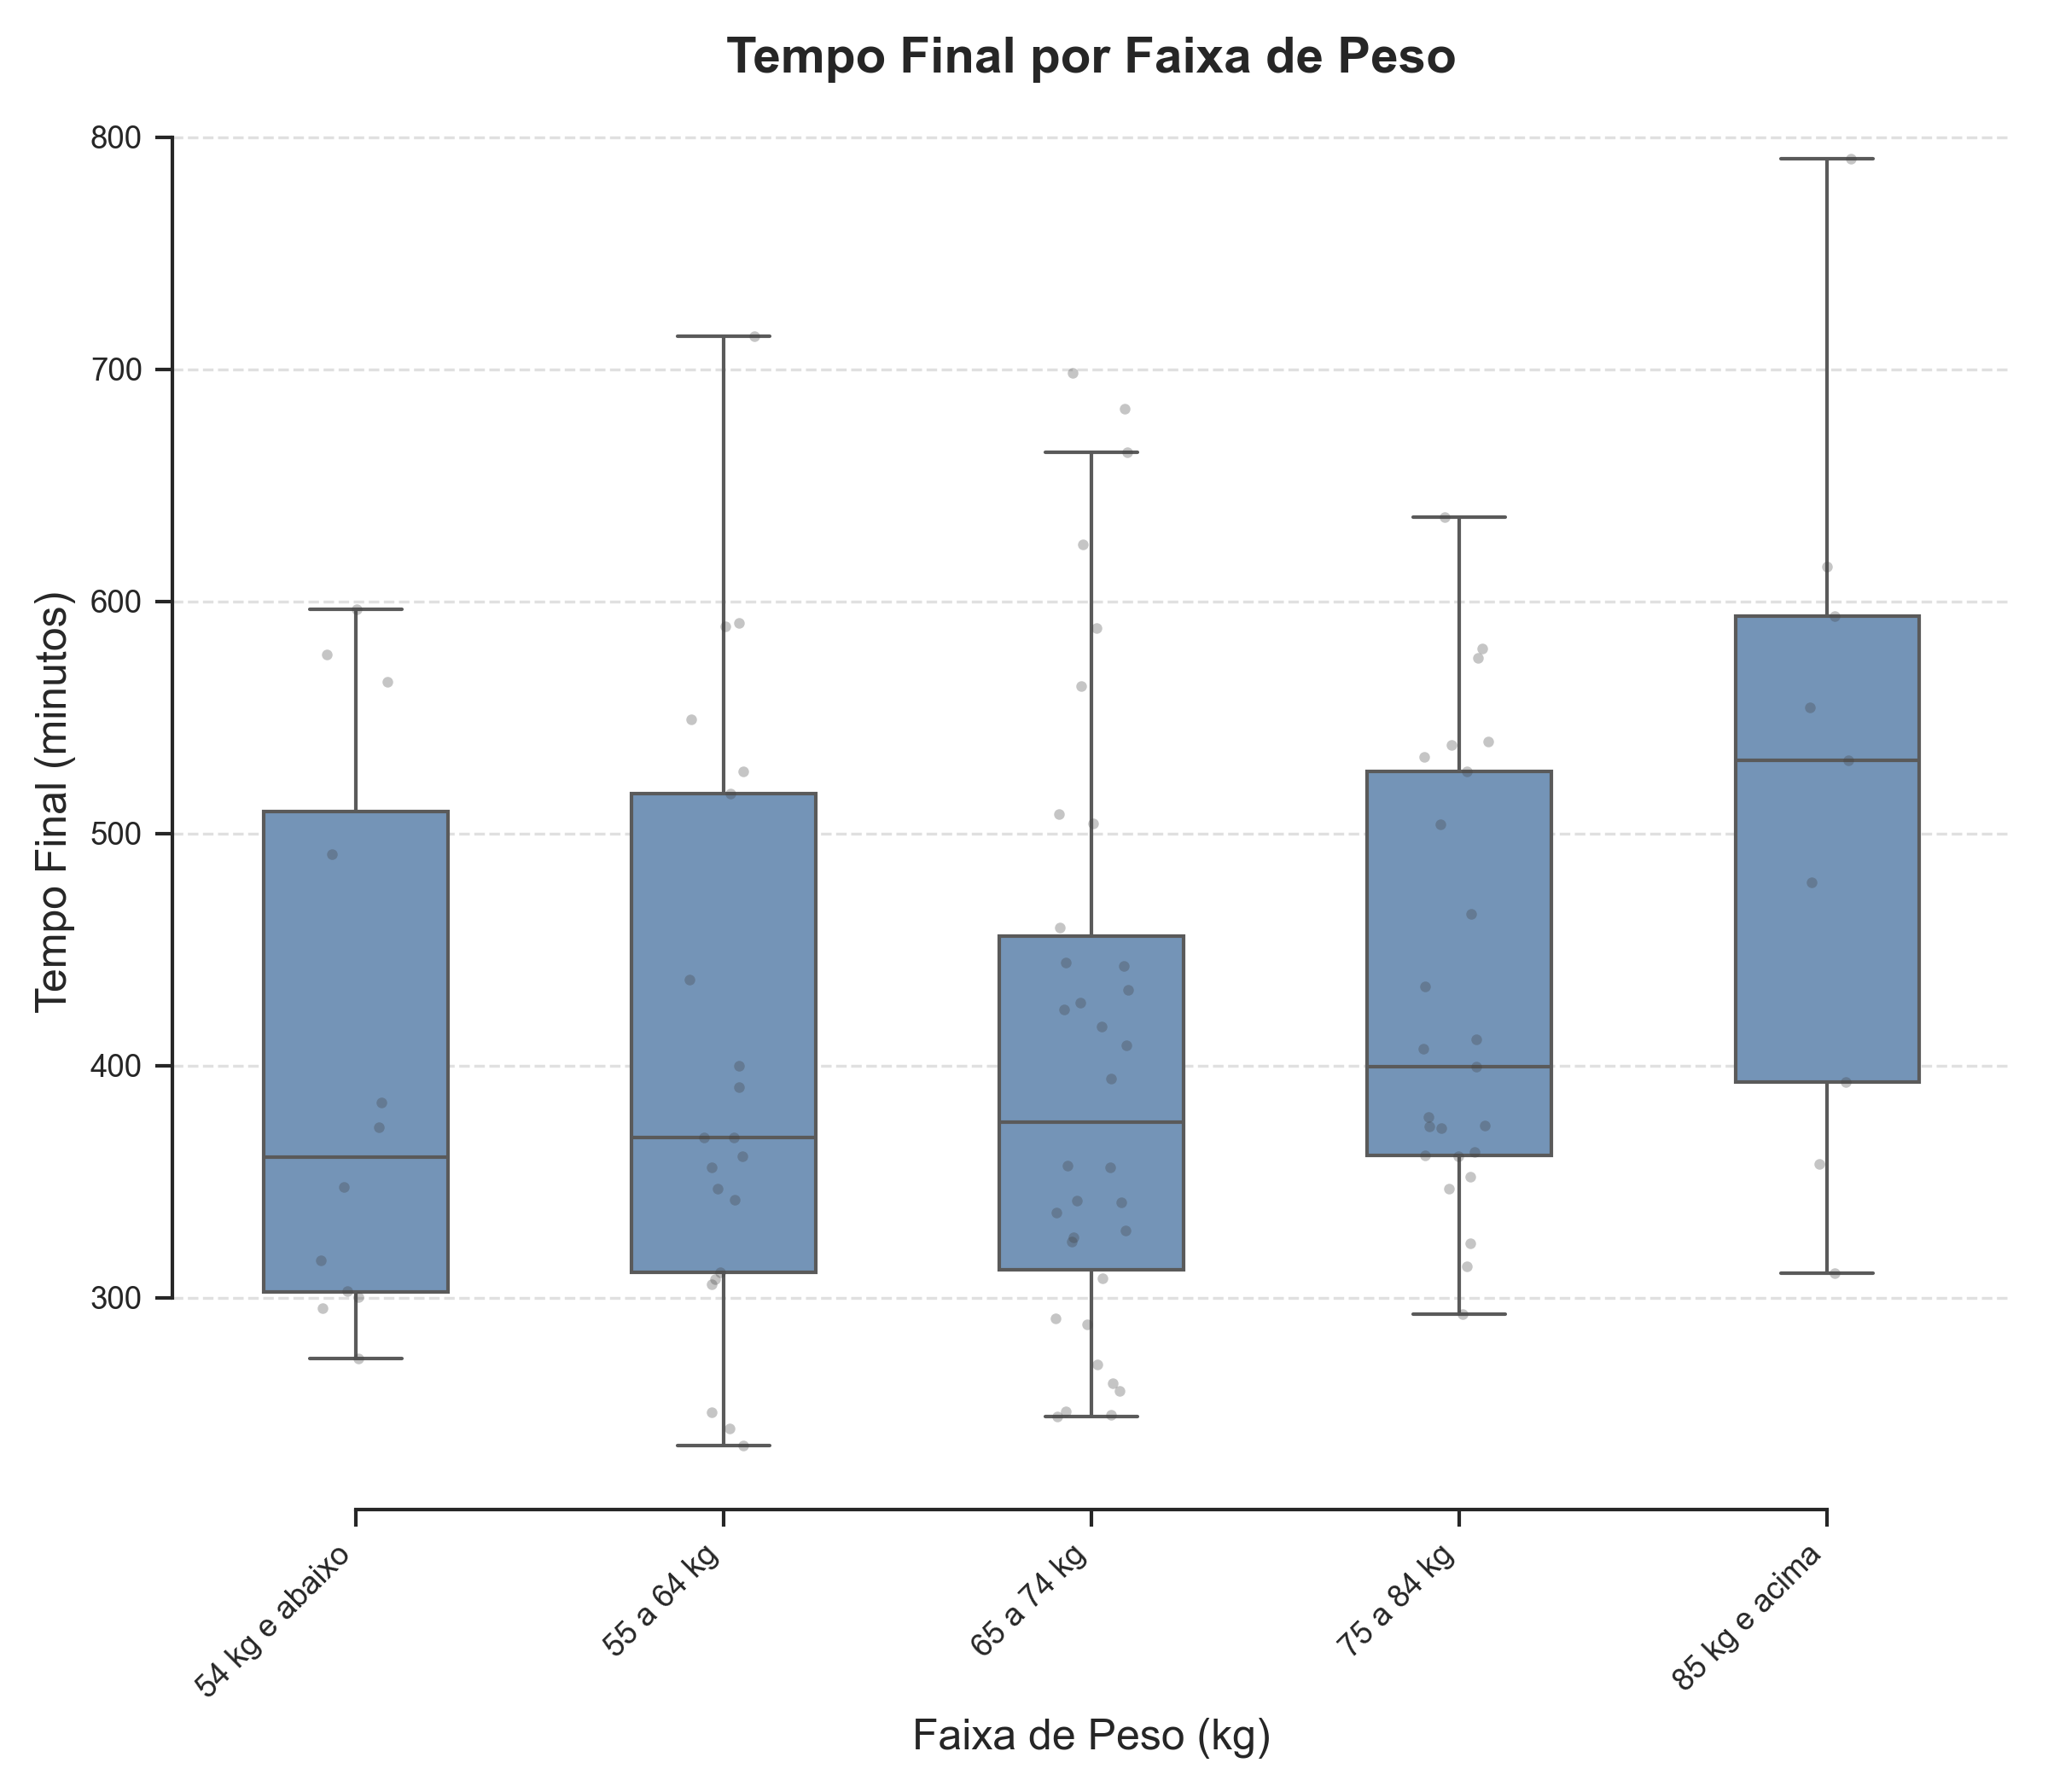
\includegraphics[width=0.8\textwidth]{Imagens/boxplot_tempo_por_peso.png}
    \caption{Boxplot comparativo do Tempo Final por Faixa de Peso.}
    \label{fig:boxplot_peso}
    \caption*{Fonte: Elaborado pelo autor (2025).}
\end{figure}

\section{Análise da Consistência de Ritmo}

A análise da relação entre a consistência do ritmo (\texttt{Variabilidade\_Ritmo\_min\_std}) e o desempenho (\texttt{Tempo\_Final\_min}) foi um ponto central do estudo. Como ambas as variáveis não apresentaram distribuição normal (Shapiro-Wilk com p<0.001 para ambas), optou-se pela \textbf{Correlação de Spearman}.

O resultado revelou um coeficiente \textbf{rho ($\rho$) de 0.9388} com um \textbf{p-valor virtualmente zero ($p \approx 2.44 \times 10^{-51}$)}. Isso indica uma \textbf{correlação positiva muito forte e significativa}. A Figura \ref{fig:scatter_variabilidade} ilustra essa relação de forma clara.

% --- Figura Scatter Plot Variabilidade ---
% COMENTÁRIO: João, insira aqui o arquivo de imagem do seu scatter plot (In [40]).
\begin{figure}[H]
    \centering
    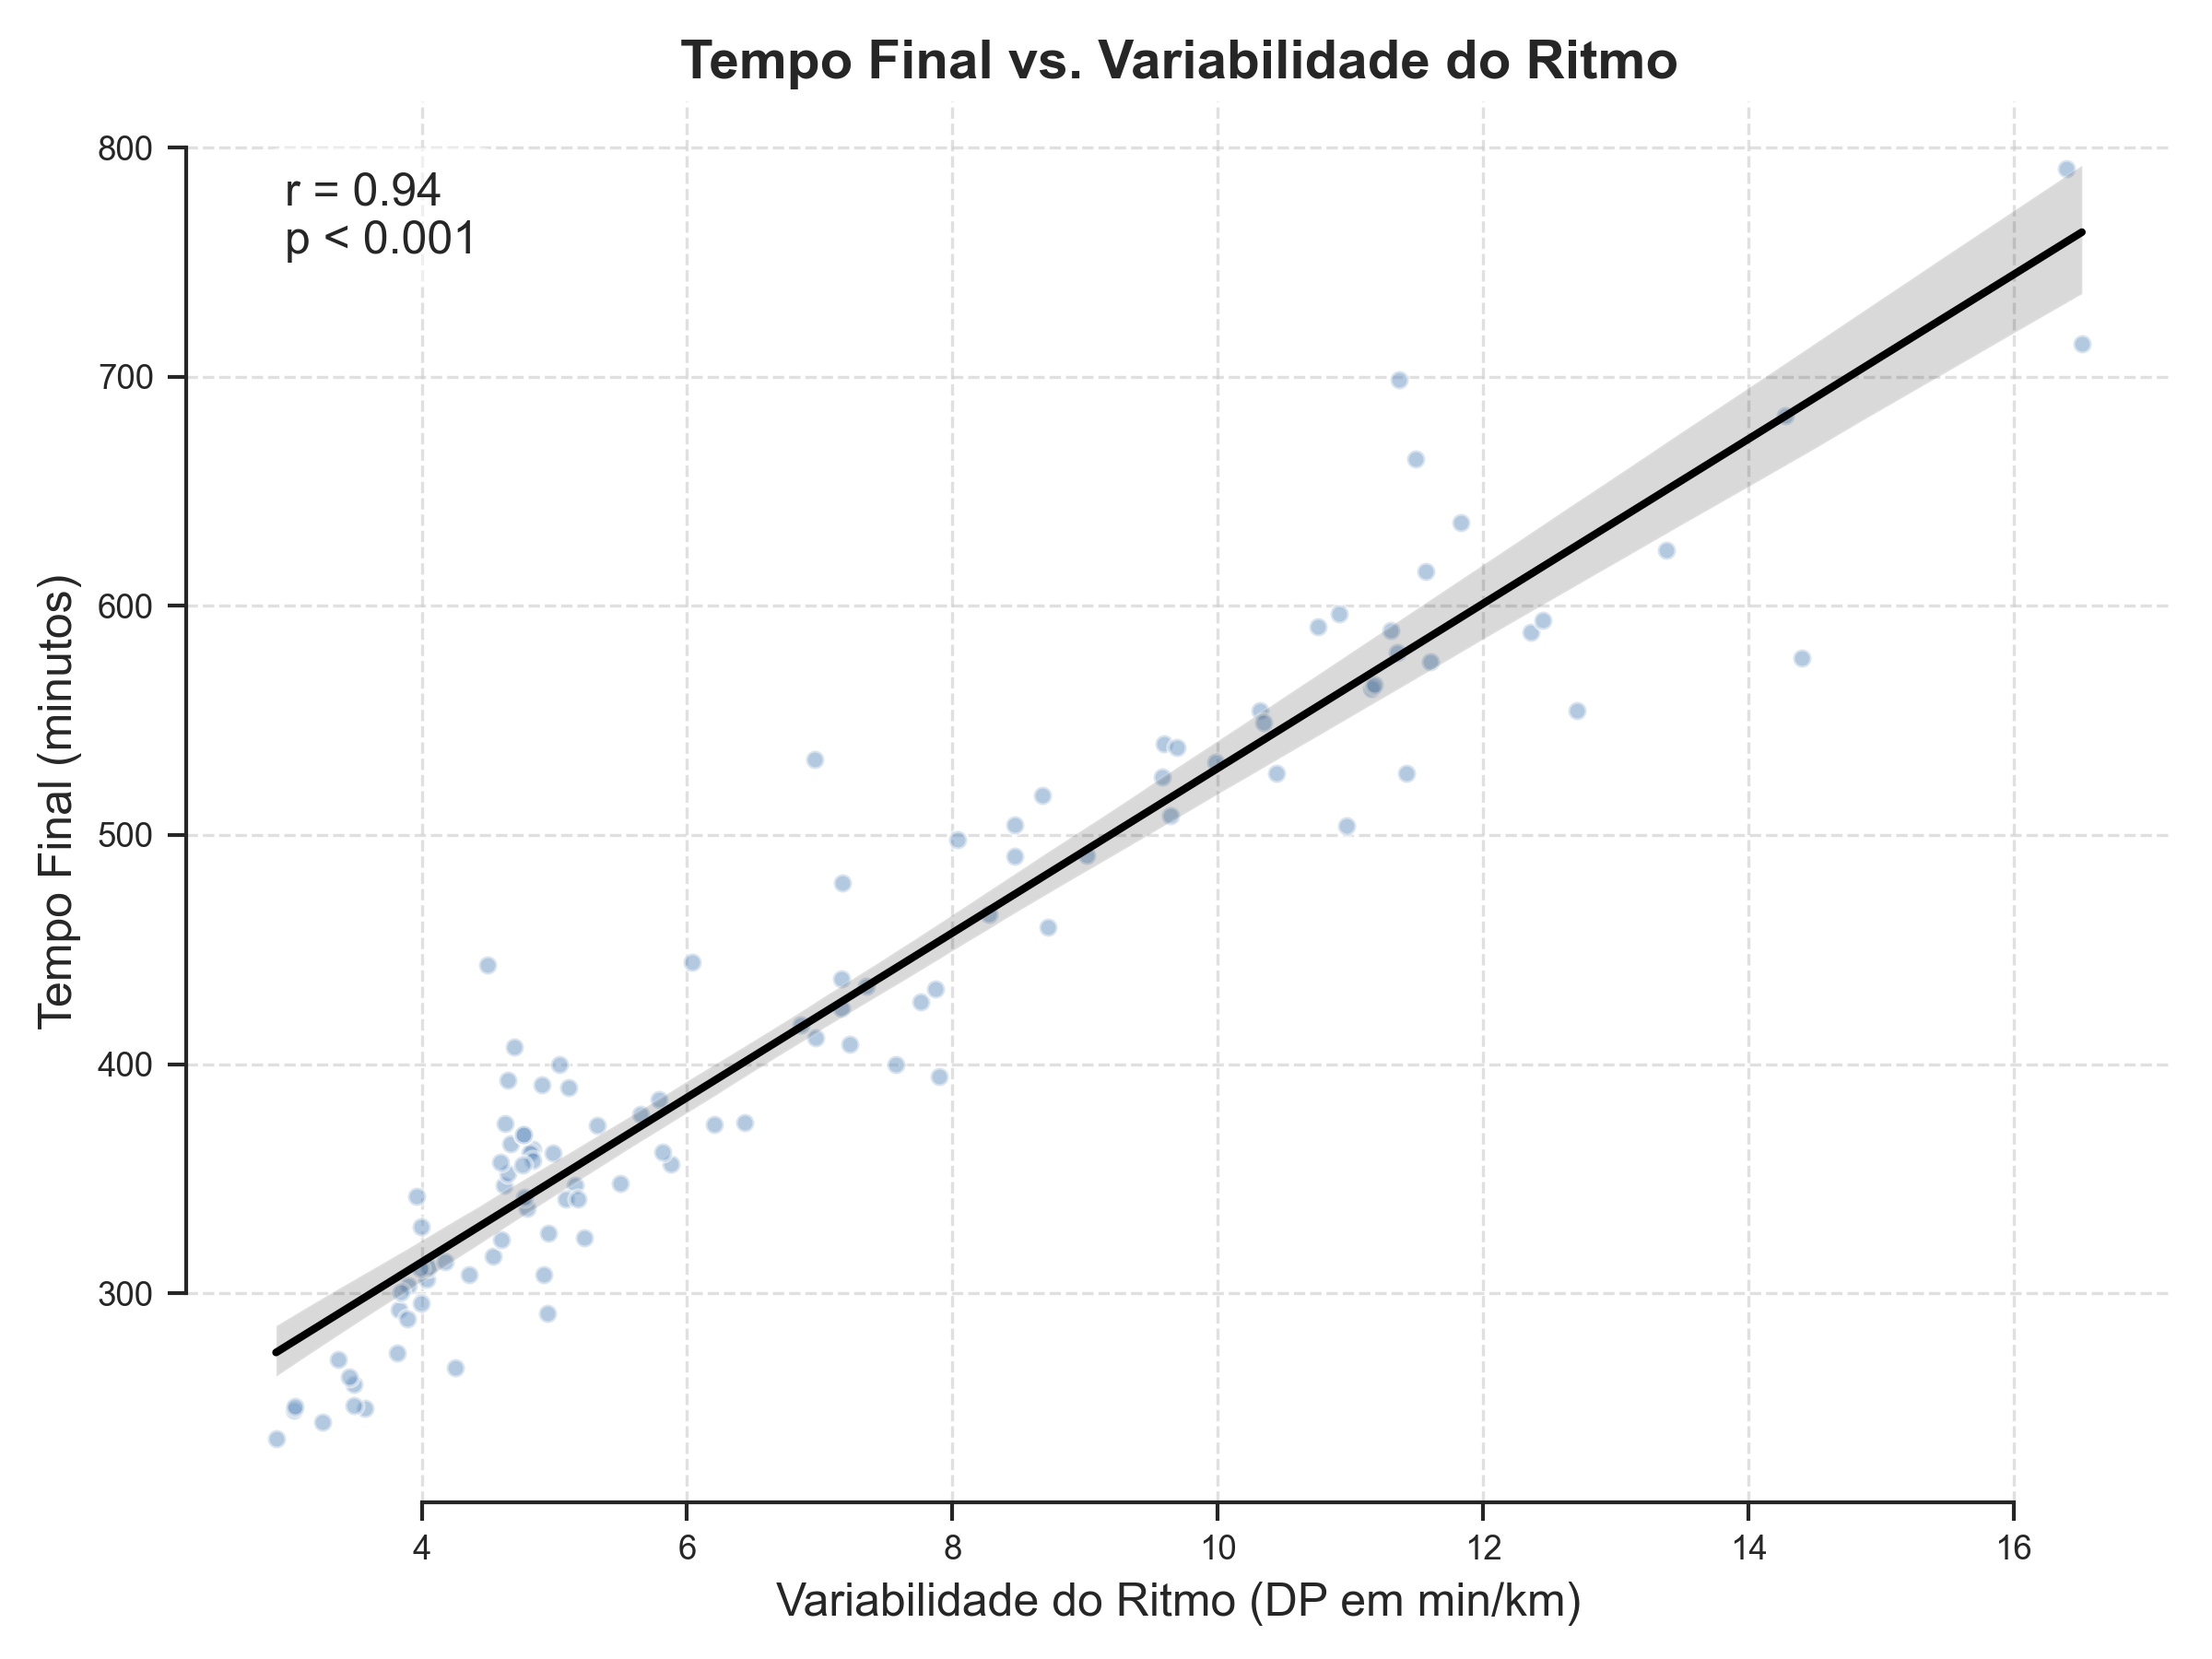
\includegraphics[width=0.8\textwidth]{Imagens/scatterplot_correlacao_ritmo.png}
    \caption{Gráfico de dispersão entre a Variabilidade do Ritmo e o Tempo Final.}
    \label{fig:scatter_variabilidade}
    \caption*{Fonte: Elaborado pelo autor (2025).}
\end{figure}

\textbf{Interpretação:} A forte correlação positiva confirma que atletas que mantiveram um ritmo mais constante ao longo da prova (menor desvio padrão) tenderam a obter tempos finais melhores (menores). A consistência do ritmo, portanto, emerge como um fator preditivo fundamental do desempenho.

\section{Análise de Agrupamento: As Personas dos Corredores}

Com o objetivo de identificar perfis de atletas com estratégias e habilidades distintas, foi realizada uma análise de clusterização K-Means. A seleção do número de clusters foi guiada pelo Método do Cotovelo, que indicou k=4 como o número ideal de agrupamentos. As variáveis utilizadas na clusterização foram selecionadas para capturar múltiplas dimensões da performance, incluindo: desempenho geral (\texttt{Tempo\_Final\_seg}), consistência (\texttt{Variabilidade\_Ritmo\_std}), gestão de prova (\texttt{diff\_relativa\_segunda\_primeira\_parte}) e especialização em terreno (\texttt{indice\_subida}, \texttt{indice\_descida}).
A análise das características médias de cada grupo (Tabela \ref{tab:perfis_clusters}) e a visualização de suas distribuições (Figura \ref{fig:boxplot_clusters}) permitiram a definição de quatro "personas" distintas de corredores.

% --- Tabela Perfis dos Clusters ---
\begin{table}[H]
\centering
\caption{Perfil médio das variáveis chave para cada cluster (k=4).}
\label{tab:perfis_clusters}
\resizebox{1.05\textwidth}{!}{%
\begin{tabular}{lccccc}
\toprule
\textbf{Variável} & \textbf{Cluster 0 (Escaladores)} & \textbf{Cluster 1 (Especialistas em Descidas)} & \textbf{Cluster 2 (Guerreiros)} & \textbf{Cluster 3 (Elite)} \\
\midrule
Tempo\_Final\_seg & 22871.56 & 30604.38 & 37286.06 & 18056.06 \\
Variabilidade\_Ritmo\_std & 325.15 & 582.33 & 711.45 & 258.11 \\
diff\_relativa... & -0.15 & -0.12 & -0.13 & -0.22 \\
indice\_subida & 0.19 & 0.28 & 0.22 & 0.20 \\
indice\_descida & -0.13 & -0.22 & -0.17 & -0.15 \\
\bottomrule
\end{tabular}
}
\caption*{Fonte: Elaborado pelo autor (2025).}
\end{table}

% --- Figura Boxplots por Cluster ---
% COMENTÁRIO: João, insira aqui o arquivo de imagem da sua grade de boxplots (In [120]).
\begin{figure}[H]
    \centering
    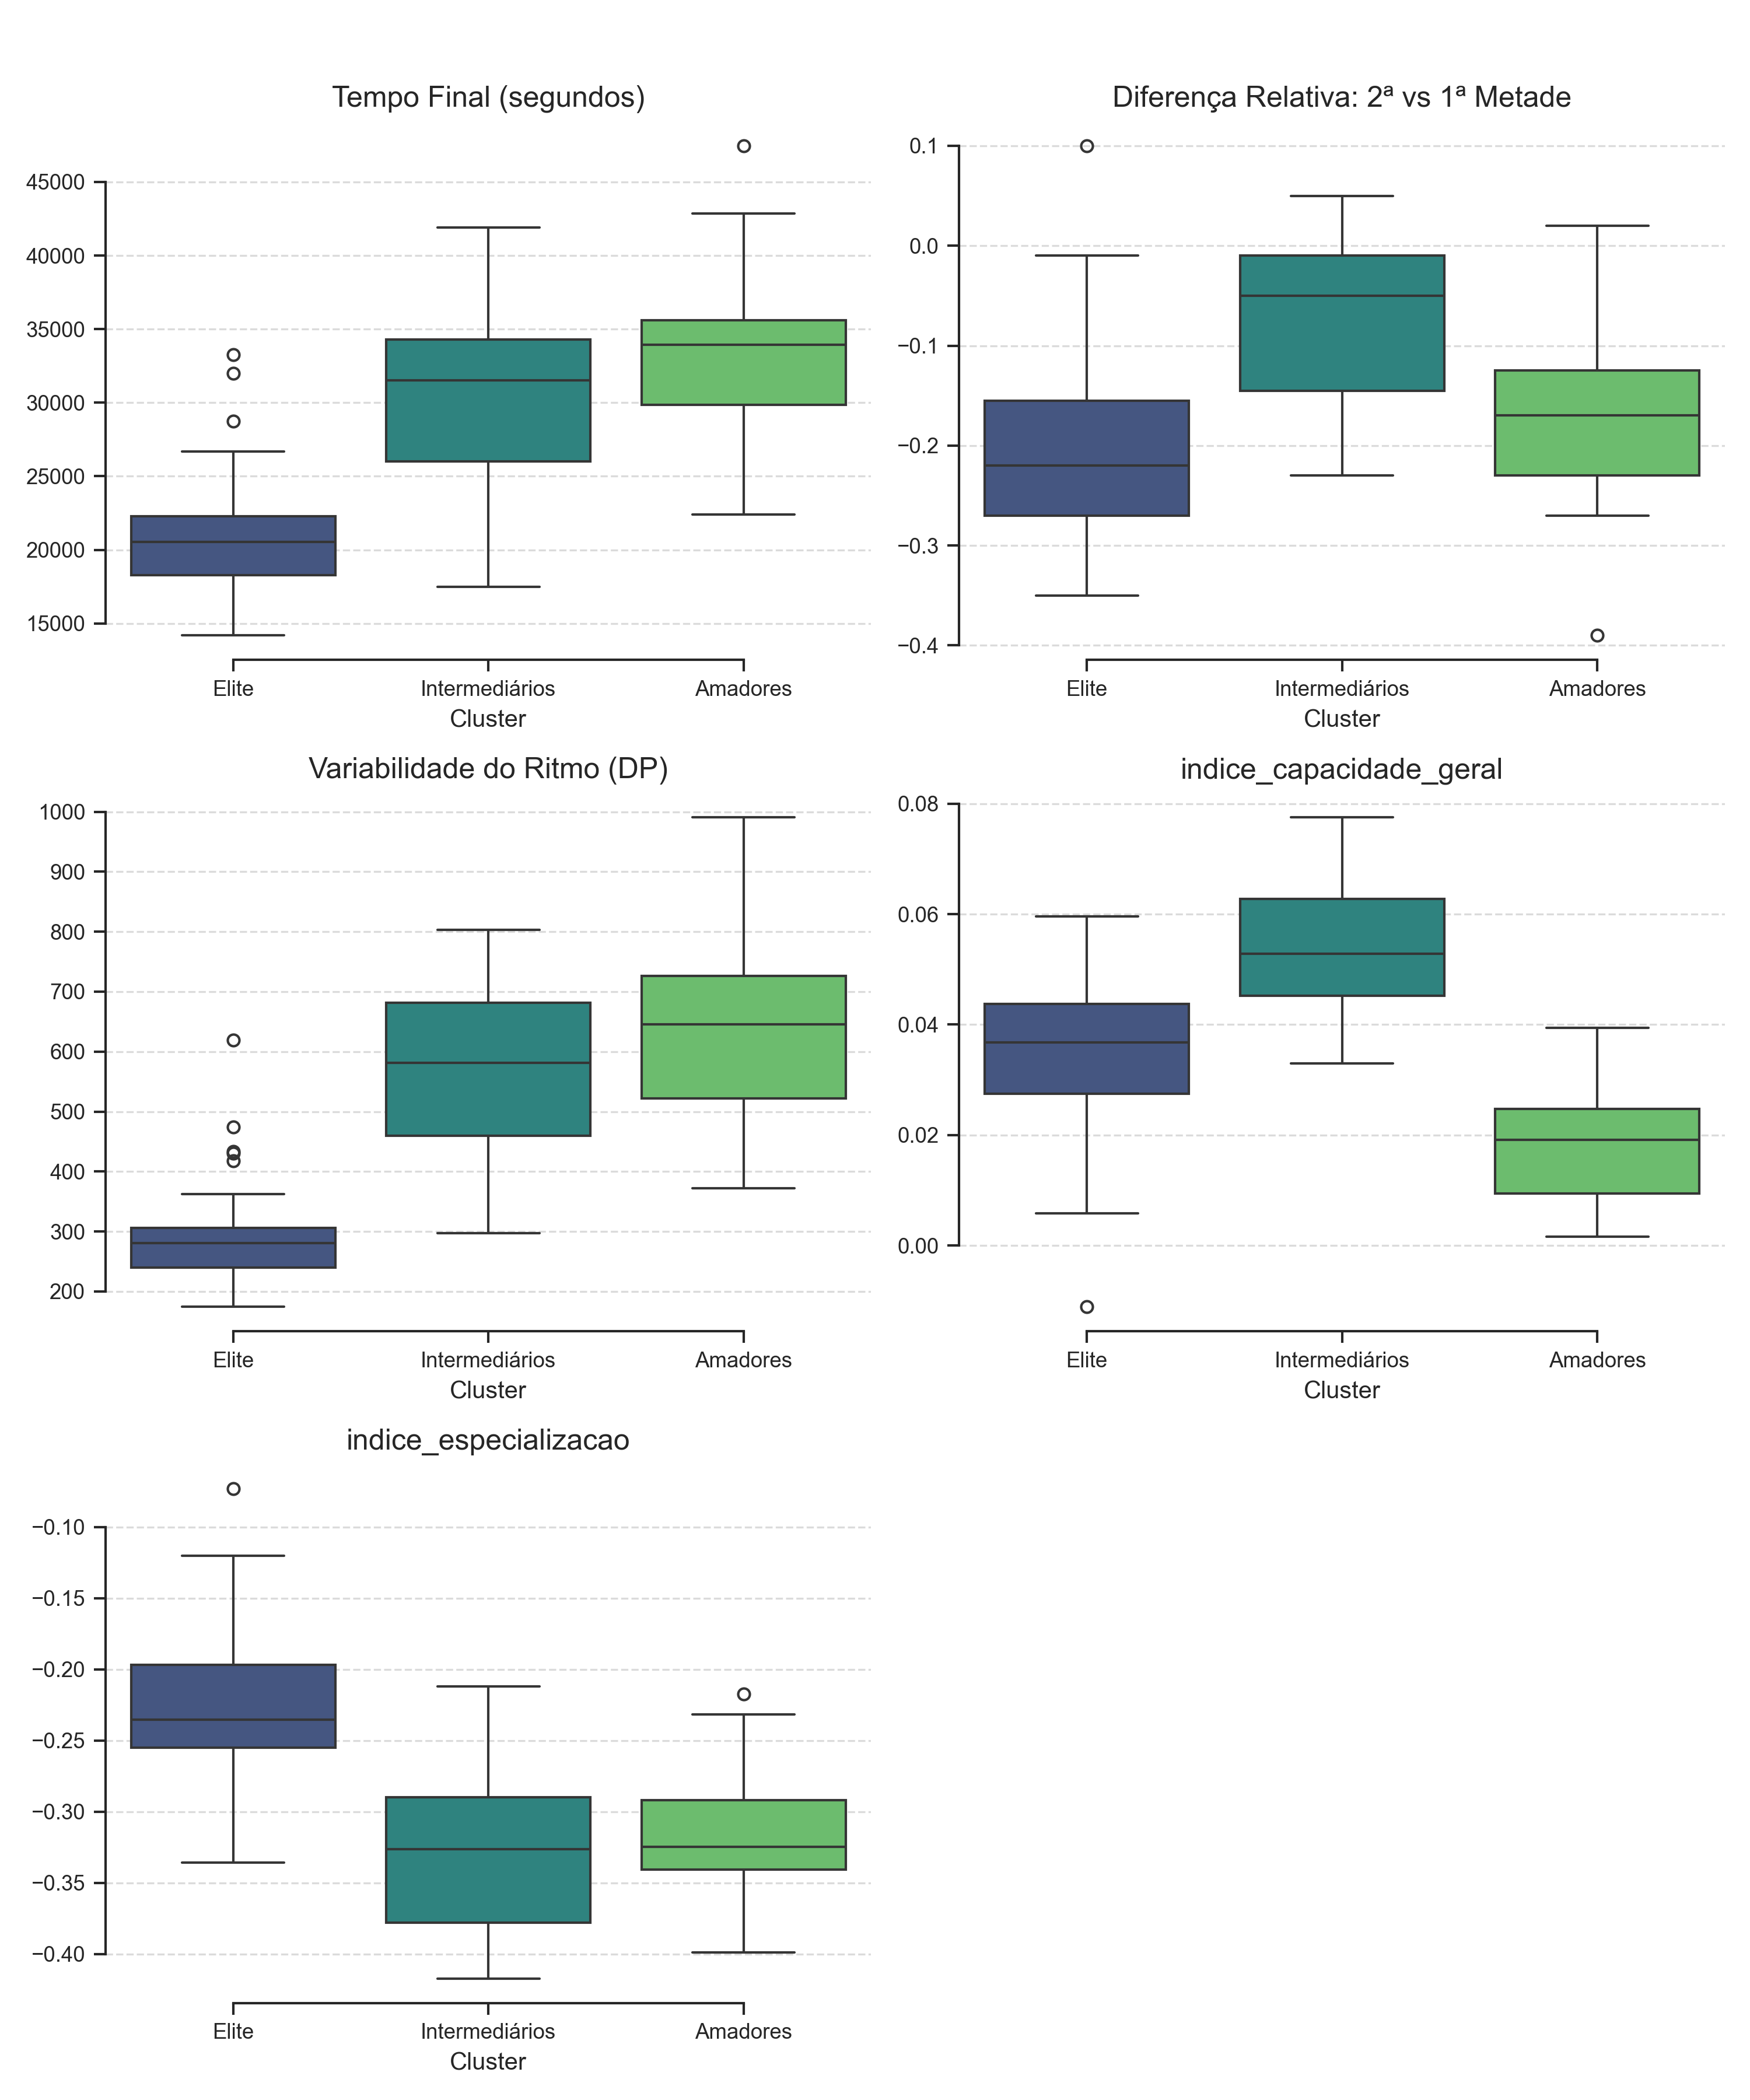
\includegraphics[width=1.05\textwidth]{Imagens/boxplot_clusters_features.png}
    \caption{Distribuição das variáveis chave por cluster.}
    \label{fig:boxplot_clusters}
    \caption*{Fonte: Elaborado pelo autor (2025).}
\end{figure}

\begin{itemize}
    \item \textbf{Cluster 3 (34 atletas): A Elite Completa.} Este grupo apresentou o menor tempo final (média de \textbf{5 horas e 56 segundos}), a menor variabilidade de ritmo e a melhor gestão de prova (\texttt{diff\_relativa} mais negativa). Seus índices de subida e descida são excelentes, demonstrando proficiência em todos os terrenos. Persona: Rápidos, estratégicos e tecnicamente completos.
    \item \textbf{Cluster 0 (34 atletas): Os Escaladores.} O segundo grupo mais rápido (média de \textbf{6 horas, 21 minutos e 11 segundos}). Sua principal característica é o excepcional desempenho em subidas, possuindo o melhor \texttt{indice\_subida} (0.19), mas um desempenho apenas mediano em descidas (\texttt{indice\_descida} de -0.13). Persona: Usam a força na subida como principal arma.
    \item \textbf{Cluster 1 (24 atletas): Os Especialistas em Descida.} Grupo intermediário (média de \textbf{8 horas, 30 minutos e 4 segundos}). Caracterizam-se por terem o pior desempenho relativo em subidas (\texttt{indice\_subida} de 0.28), mas o melhor desempenho em descidas (\texttt{indice\_descida} de -0.22). Sua alta variabilidade de ritmo é explicada por essa grande diferença de performance entre os terrenos. Persona: Atletas tecnicamente hábeis que compensam nas descidas o tempo perdido nas subidas.
    \item \textbf{Cluster 2 (17 atletas): Os Guerreiros.} O grupo com o maior tempo final (média de \textbf{10 horas, 21 minutos e 26 segundos}) e a maior variabilidade de ritmo. Seus índices de subida e descida são equilibrados, mas em um patamar de performance geral inferior. Persona: Focados em completar o desafio, com um perfil de resistência em vez de especialização técnica.
\end{itemize}

\section{Modelo Preditivo do Desempenho}

Para unificar os achados anteriores, foi ajustado um modelo de Regressão Linear Múltipla tendo o \texttt{Tempo\_Final\_seg} como variável dependente. Utilizando um processo de eliminação retrógrada (\textit{backward elimination}), buscou-se um modelo final parcimonioso e robusto, removendo-se as variáveis não significativas. O modelo final, apresentado na Tabela \ref{tab:modelo_regressao}, reteve apenas as variáveis com poder explicativo estatisticamente significativo.

% --- Tabela do Modelo Final ---
\begin{table}[H]
\centering
\caption{Sumário do Modelo Final de Regressão Linear Múltipla (OLS).}
\label{tab:modelo_regressao}
\begin{tabular}{lrrrr}
\toprule
\textbf{Variável} & \textbf{Coef.} & \textbf{Erro Padrão} & \textbf{t} & \textbf{P>|t|} \\
\midrule
\textbf{Intercepto} & 14990.00 & 620.56 & 24.15 & <0.001 \\
\texttt{Variabilidade\_Ritmo\_std} & 24.25 & 1.71 & 14.16 & <0.001 \\
\texttt{cluster\_1} & 1496.91 & 612.66 & 2.44 & 0.016 \\
\texttt{cluster\_2} & 5047.70 & 814.12 & 6.20 & <0.001 \\
\texttt{cluster\_3} & -3189.92 & 404.11 & -7.89 & <0.001 \\
\midrule
\multicolumn{5}{l}{\textbf{R² Ajustado:} 0.953} \\
\multicolumn{5}{l}{\textbf{Prob (F-statistic):} 5.55e-69} \\
\bottomrule
\end{tabular}
\caption*{Fonte: Elaborado pelo autor (2025).}
\end{table}

O modelo final apresentou um \textbf{R² ajustado de 0.953}, indicando que 95.3\% da variabilidade no tempo final dos atletas é explicada pelas variáveis do modelo. O Teste F global foi altamente significativo ($p \approx 5.55 \times 10^{-69}$), validando a significância do modelo como um todo. A interpretação dos coeficientes revela dois pilares do desempenho:
\begin{enumerate}
    \item \textbf{Consistência do Ritmo (\texttt{Variabilidade\_Ritmo\_std}):} Com um coeficiente de \textbf{24.25 (p<0.001)}, o modelo quantifica que para cada 1 segundo de aumento no desvio padrão do ritmo, o tempo final de prova aumenta, em média, em 24.25 segundos.
    \item \textbf{Perfil do Atleta (\texttt{cluster}):} As variáveis dummy dos clusters foram altamente significativas. Tomando o Cluster 0 ("Os Escaladores") como referência:
    \begin{itemize}
        \item Pertencer ao \textbf{Cluster 3 ("A Elite")} está associado a uma redução de \textbf{3.190 segundos} (aprox. 53 minutos) no tempo final (p<0.001).
        \item Pertencer ao \textbf{Cluster 1 ("Especialistas em Descida")} está associado a um aumento de \textbf{1.497 segundos} (aprox. 25 minutos) no tempo final (p=0.016).
        \item Pertencer ao \textbf{Cluster 2 ("Guerreiros")} está associado a um aumento de \textbf{5.048 segundos} (aprox. 84 minutos) no tempo final (p<0.001).
    \end{itemize}
\end{enumerate}
É notável que, após a inclusão da variável \texttt{cluster}, as variáveis demográficas como \texttt{sexo} e \texttt{faixa\_etaria} perderam significância e foram removidas do modelo final. Isso sugere que a variável \texttt{cluster} captura de forma mais eficaz e completa as diferenças de desempenho.

\section{Análise de Resíduos do Modelo Final}

A validação dos pressupostos do modelo de regressão foi realizada por meio da análise de seus resíduos.

% --- Figuras da Análise de Resíduos ---
% COMENTÁRIO: João, insira aqui os dois gráficos de análise de resíduos (In [3496]).
\begin{figure}[H]
    \centering
    \begin{minipage}{1\textwidth}
        \centering
        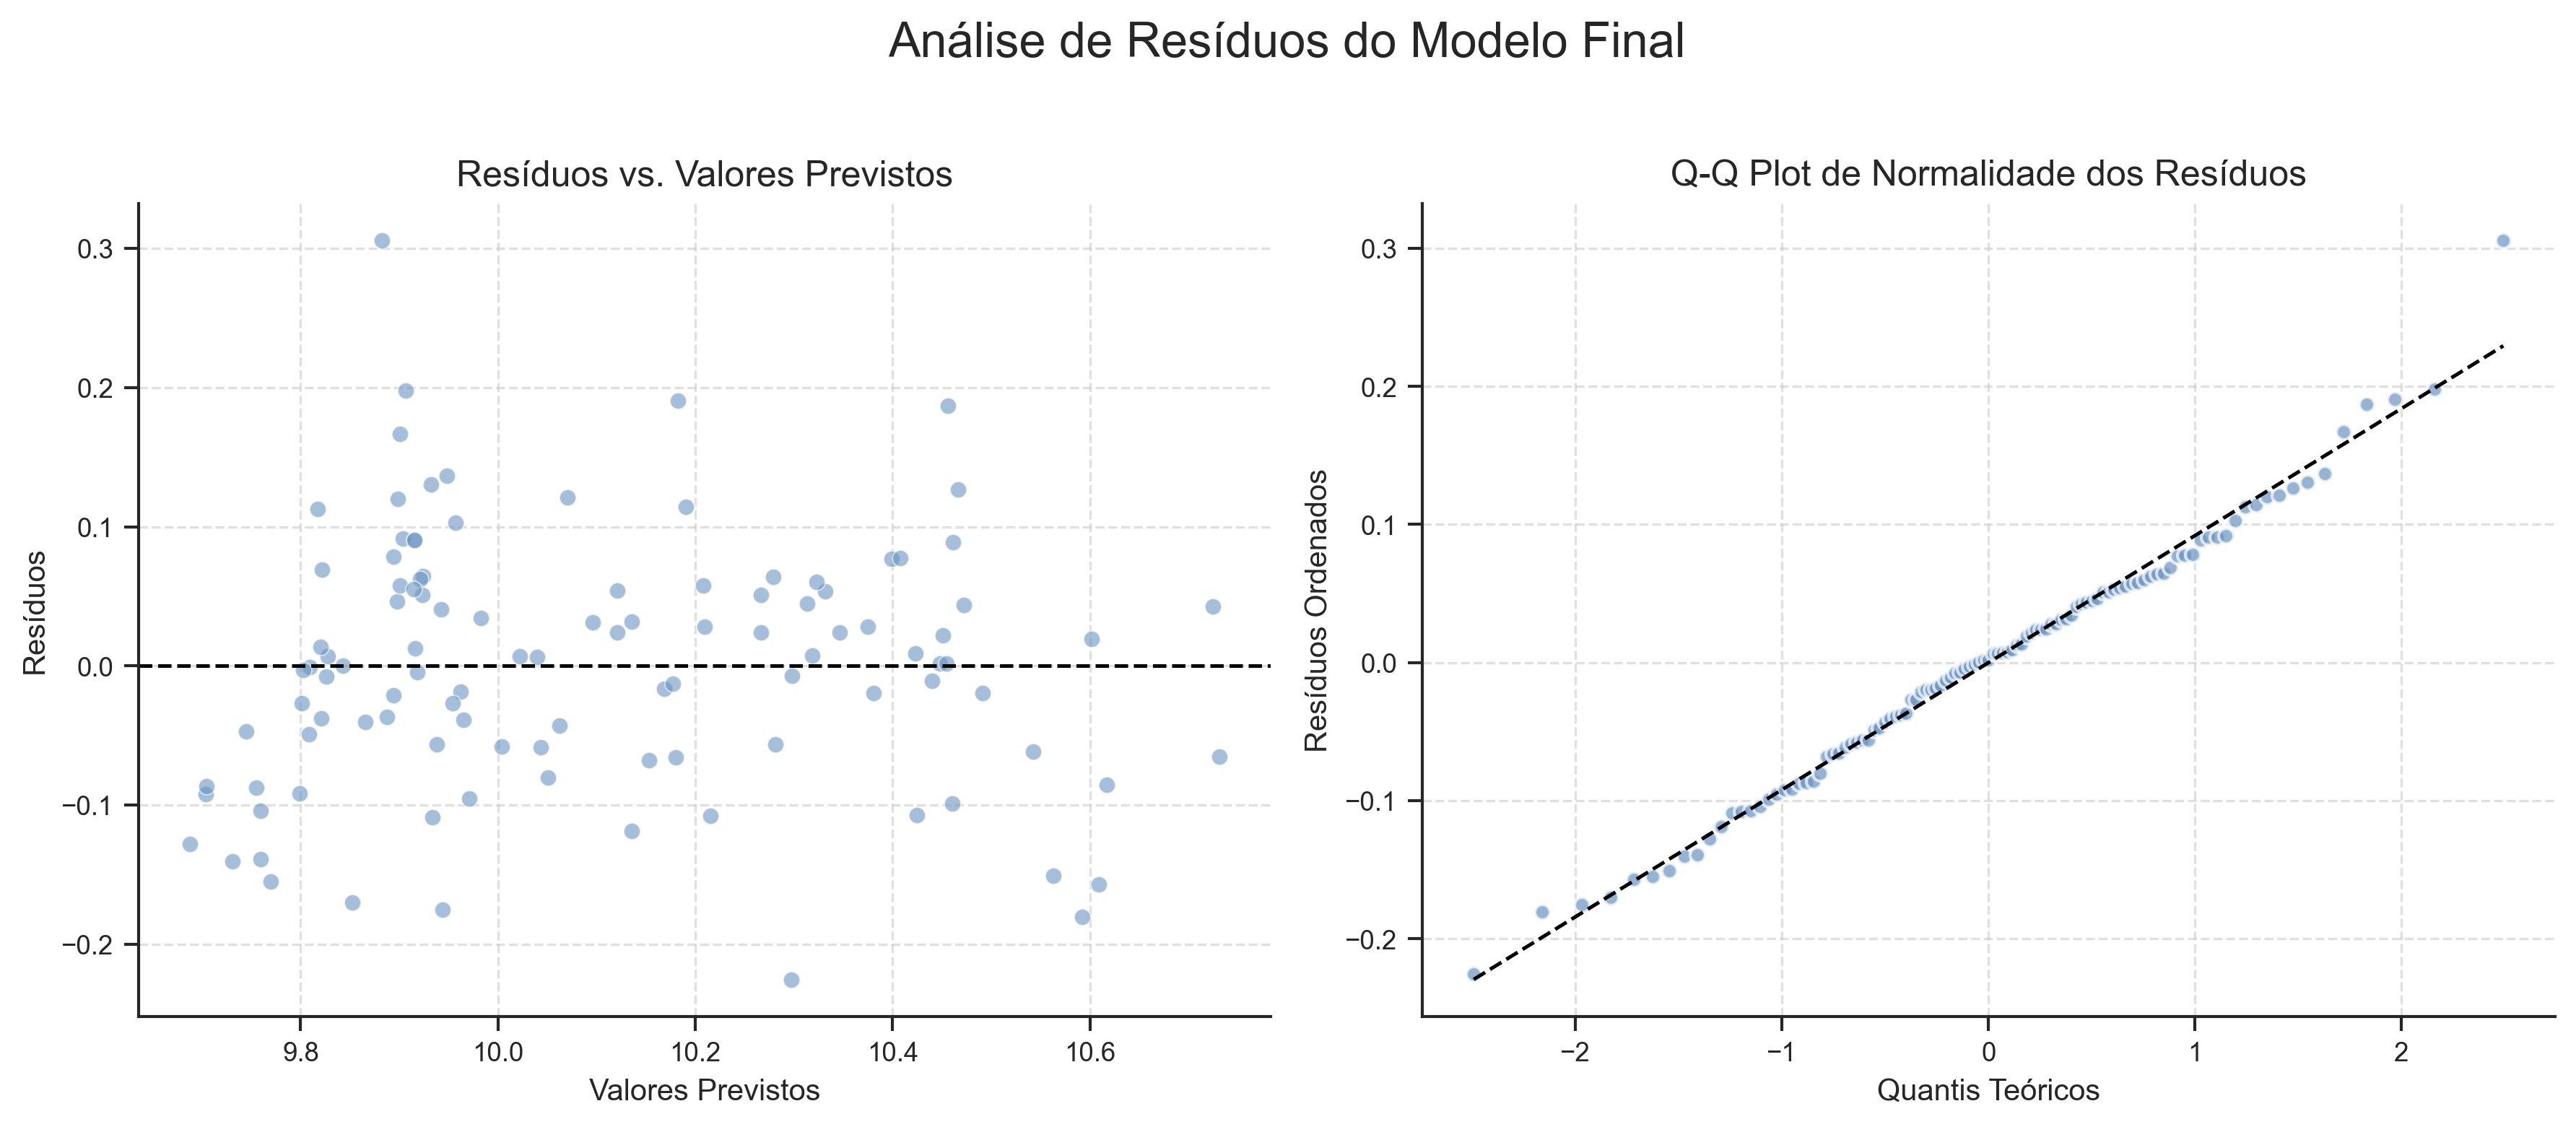
\includegraphics[width=\linewidth]{Imagens/analise_residuos_modelo.png}
        \caption{Resíduos vs. Valores Previstos.}
        \label{fig:residuos}
    \end{minipage}\hfill
    \caption*{Fonte: Elaborado pelo autor (2025).}
\end{figure}

\begin{itemize}
    \item \textbf{Linearidade e Homocedasticidade:} O gráfico de resíduos versus valores previstos (Figura \ref{fig:residuos}) exibe uma nuvem de pontos aleatoriamente dispersa em torno da linha zero, sem padrões discerníveis. Isso indica que os pressupostos de linearidade e homocedasticidade foram satisfeitos.
    \item \textbf{Independência dos Resíduos:} O valor do teste de \textbf{Durbin-Watson foi de 1.981}, muito próximo de 2, indicando ausência de autocorrelação serial nos resíduos.
    \item \textbf{Normalidade dos Resíduos:} O gráfico Q-Q (Figura \ref{fig:residuos}) mostra que, embora os pontos centrais se alinhem bem à reta teórica, há desvios nas caudas. Isso, em conjunto com os testes de Omnibus (p=0.008) e Jarque-Bera (p=0.008), confirma que o \textbf{pressuposto de normalidade dos resíduos foi violado}. Essa violação pode afetar a precisão dos intervalos de confiança e dos p-valores. Contudo, dado o altíssimo poder explicativo do modelo (R² > 0.95) e a forte significância dos preditores, as conclusões práticas sobre a importância da consistência e dos perfis de atleta permanecem robustas.
\end{itemize}

\end{document}

    %====================================================================
    % Referências bibliográficas
    %====================================================================
    \newpage
    \def\thispagestyle#1{}
    %\bibliographystyle{babplain-fl}
    \bibliographystyle{plainnat}
    \bibliography{Bibliografia/bibliografia}

    
    %====================================================================
    % Apêndices da monografia
    % Pode ser que o trabalho tenha vários apêndices. Coloque os 
    % apêndices em uma pasta e dentro da pasta %crie o arquivo tex com o 
    % texto associado ao apêndice. 
    %====================================================================
    %\begin{appendices}
    %\input{apendices/apendice1/apendice1.tex}
    %\input{apendices/apendice2/apendice2.tex}
    %\end{appendices}

    \end{document}
